%%
%% This is file `sigconf.tex',
%% generated with the docstrip utility.
%%
%% The original source files were:
%%
%% samples.dtx  (with options: `all,proceedings,sigconf')
%% 
%% IMPORTANT NOTICE:
%% 
%% For the copyright see the source file.
%% 
%% Any modified versions of this file must be renamed
%% with new filenames distinct from sigconf.tex.
%% 
%% For distribution of the original source see the terms
%% for copying and modification in the file samples.dtx.
%% 
%% This generated file may be distributed as long as the
%% original source files, as listed above, are part of the
%% same distribution. (The sources need not necessarily be
%% in the same archive or directory.)
%%
%%
%% Commands for TeXCount
%TC:macro \cite [option:text,text]
%TC:macro \citep [option:text,text]
%TC:macro \citet [option:text,text]
%TC:envir table 0 1
%TC:envir table* 0 1
%TC:envir tabular [ignore] word
%TC:envir displaymath 0 word
%TC:envir math 0 word
%TC:envir comment 0 0
%%
%% The first command in your LaTeX source must be the \documentclass
%% command.
%%
%% For submission and review of your manuscript please change the
%% command to \documentclass[manuscript, screen, review]{acmart}.
%%
%% When submitting camera ready or to TAPS, please change the command
%% to \documentclass[sigconf]{acmart} or whichever template is required
%% for your publication.
%%
%%
\documentclass[sigconf]{acmart}
% ---------- Packages ----------
\usepackage{amsmath}
% amssymb intentionally omitted: newtxmath (loaded by acmart) already
% provides the AMS symbol set, and the two packages collide on \Bbbk.
\usepackage{amsthm}
\usepackage{mathrsfs}
\usepackage{booktabs}
\usepackage{multirow}
\usepackage{array}
\usepackage{xcolor}
\usepackage{tikz}
\usetikzlibrary{positioning, arrows.meta, calc, shapes, fit, backgrounds, shadows.blur, decorations.pathreplacing, decorations.pathmorphing}
\usepackage[utf8]{inputenc}
\usepackage[T1]{fontenc}
\usepackage{microtype}
\usepackage{enumitem}
\usepackage{listings}
\usepackage{xspace}
\usepackage{algorithm}
\usepackage{algpseudocode}

% ---------- Color palette (matches presentation) ----------
% Softer / warmer than the original SIGMOD deck, aligned with the
% OptAMI reference style: brick-red highlights, warm tan and olive
% accents against a deep navy backbone and cream surface.
\definecolor{mosaicCrimson}{HTML}{A0252A}
\definecolor{mosaicBlue}{HTML}{003049}
\definecolor{mosaicLightBlue}{HTML}{669BBC}
\definecolor{mosaicCream}{HTML}{FDF0D5}
\definecolor{mosaicRed}{HTML}{C1121F}
\definecolor{mosaicGray}{HTML}{8D99AE}
\definecolor{mosaicTan}{HTML}{E5C595}    % warm tan accent (reference "Online")
\definecolor{mosaicOlive}{HTML}{A5C088}  % soft olive accent (reference "Shared")

% ---------- Listings (SQL code blocks in Section 5) ----------
\lstset{
  basicstyle=\ttfamily\small,
  keywordstyle=\color{mosaicBlue}\bfseries,
  commentstyle=\color{mosaicGray}\itshape,
  stringstyle=\color{mosaicCrimson},
  showstringspaces=false,
  breaklines=true,
  breakatwhitespace=true,
  columns=fullflexible,
  keepspaces=true,
  numbers=none,
  frame=single,
  rulecolor=\color{mosaicLightBlue},
  framesep=4pt,
  xleftmargin=2pt,
  xrightmargin=2pt,
  aboveskip=8pt,
  belowskip=8pt,
  language=SQL
}

% ---------- Theorem-like environments ----------
\theoremstyle{plain}
\newtheorem{theorem}{Theorem}
\newtheorem{lemma}[theorem]{Lemma}
\newtheorem{corollary}[theorem]{Corollary}
\newtheorem{proposition}[theorem]{Proposition}

\theoremstyle{definition}
\newtheorem{definition}{Definition}

\newtheorem{counterexample}{Counterexample}

% Proof is built-in; redefine QED
\renewcommand{\qedsymbol}{\ensuremath{\blacksquare}}

% ---------- Notation shortcuts ----------
\newcommand{\vect}[1]{\boldsymbol{#1}}
\newcommand{\attr}[1]{\operatorname{attr}(#1)}
\newcommand{\Mem}{\mathit{Mem}}
\newcommand{\KG}{\mathit{KG}}
\newcommand{\schema}[1]{\operatorname{schema}(#1)}
\newcommand{\setof}[1]{\operatorname{set}(#1)}
\newcommand{\topK}{\operatorname{topK}}
\newcommand{\bm}[1]{\boldsymbol{#1}}
\newcommand{\ie}{\emph{i.e.,}\xspace}
\newcommand{\eg}{\emph{e.g.,}\xspace}
\newcommand{\etc}{\emph{etc.}\xspace}
\newcommand{\wrt}{\emph{w.r.t.}\xspace}
\newcommand{\resp}{\emph{resp.,}\xspace}
\newcommand{\abbr}{\emph{abbr.,}\xspace}
\newcommand{\etal}{\emph{et al.}\xspace}
\newcommand{\btitle}[1]{\vspace{1ex}\noindent \textbf{#1}}
\newcommand{\eat}[1]{}
\newcommand{\bcirclednumber}[1]{\ding{\numexpr181+#1\relax}}

% Remark environment (used for non-blocking observations)
\theoremstyle{remark}
\newtheorem{remark}{Remark}


%% Rights management information.  This information is sent to you
%% when you complete the rights form.  These commands have SAMPLE
%% values in them; it is your responsibility as an author to replace
%% the commands and values with those provided to you when you
%% complete the rights form.
\setcopyright{acmlicensed}
\copyrightyear{2018}
\acmYear{2018}
\acmDOI{XXXXXXX.XXXXXXX}
%% These commands are for a PROCEEDINGS abstract or paper.
\acmConference[Conference acronym 'XX]{Make sure to enter the correct
  conference title from your rights confirmation email}{June 03--05,
  2018}{Woodstock, NY}
%%
%%  Uncomment \acmBooktitle if the title of the proceedings is different
%%  from ``Proceedings of ...''!
%%
%%\acmBooktitle{Woodstock '18: ACM Symposium on Neural Gaze Detection,
%%  June 03--05, 2018, Woodstock, NY}
\acmISBN{978-1-4503-XXXX-X/2018/06}


%%
%% Submission ID.
%% Use this when submitting an article to a sponsored event. You'll
%% receive a unique submission ID from the organizers
%% of the event, and this ID should be used as the parameter to this command.
%%\acmSubmissionID{123-A56-BU3}

%%
%% For managing citations, it is recommended to use bibliography
%% files in BibTeX format.
%%
%% You can then either use BibTeX with the ACM-Reference-Format style,
%% or BibLaTeX with the acmnumeric or acmauthoryear sytles, that include
%% support for advanced citation of software artefact from the
%% biblatex-software package, also separately available on CTAN.
%%
%% Look at the sample-*-biblatex.tex files for templates showcasing
%% the biblatex styles.
%%
%%
%% The majority of ACM publications use numbered citations and
%% references.  The command \citestyle{authoryear} switches to the
%% "author year" style.
%%
%% If you are preparing content for an event
%% sponsored by ACM SIGGRAPH, you must use the "author year" style of
%% citations and references.
%% Uncommenting
%% the next command will enable that style.
%%\citestyle{acmauthoryear}


%%
%% end of the preamble, start of the body of the document source.
\begin{document}

%%
%% The "title" command has an optional parameter,
%% allowing the author to define a "short title" to be used in page headers.
\title{MosaicOpt: An Algebraic Foundation for Agentic Memory Databases}

%%
%% The "author" command and its associated commands are used to define
%% the authors and their affiliations.
%% Of note is the shared affiliation of the first two authors, and the
%% "authornote" and "authornotemark" commands
%% used to denote shared contribution to the research.
\eat{\author{Ben Trovato}
\authornote{Both authors contributed equally to this research.}
\email{trovato@corporation.com}
\orcid{1234-5678-9012}
\author{G.K.M. Tobin}
\correspondingauthor
\authornotemark[1]
\email{webmaster@marysville-ohio.com}
\affiliation{%
  \institution{Institute for Clarity in Documentation}
  \city{Dublin}
  \state{Ohio}
  \country{USA}
}

\author{Lars Th{\o}rv{\"a}ld}
\affiliation{%
  \institution{The Th{\o}rv{\"a}ld Group}
  \city{Hekla}
  \country{Iceland}}
\email{larst@affiliation.org}

\author{Valerie B\'eranger}
\affiliation{%
  \institution{Inria Paris-Rocquencourt}
  \city{Rocquencourt}
  \country{France}
}

\author{Aparna Patel}
\affiliation{%
 \institution{Rajiv Gandhi University}
 \city{Doimukh}
 \state{Arunachal Pradesh}
 \country{India}}

\author{Huifen Chan}
\affiliation{%
  \institution{Tsinghua University}
  \city{Haidian Qu}
  \state{Beijing Shi}
  \country{China}}

\author{Charles Palmer}
\affiliation{%
  \institution{Palmer Research Laboratories}
  \city{San Antonio}
  \state{Texas}
  \country{USA}}
\email{cpalmer@prl.com}

\author{John Smith}
\affiliation{%
  \institution{The Th{\o}rv{\"a}ld Group}
  \city{Hekla}
  \country{Iceland}}
\email{jsmith@affiliation.org}

\author{Julius P. Kumquat}
\correspondingauthor
\affiliation{%
  \institution{The Kumquat Consortium}
  \city{New York}
  \country{USA}}
\email{jpkumquat@consortium.net}

%%
%% By default, the full list of authors will be used in the page
%% headers. Often, this list is too long, and will overlap
%% other information printed in the page headers. This command allows
%% the author to define a more concise list
%% of authors' names for this purpose.
\renewcommand{\shortauthors}{Trovato et al.}
}
%%
%% The abstract is a short summary of the work to be presented in the
%% article.
\begin{abstract}
\noindent
Production LLM agents accumulate multi-modal memory across two timescales:
long-term facts and preferences, and short-term working context. A memory
unit typically carries text, one or more dense vector embeddings,
structured metadata, and graph relations. Useful queries against this
store are conjunctive expressions that mix all four modalities, for
example, ``find passages about a fault-tolerance bug from the last 30
days, semantically similar to a stack trace, attributed to a known
subsystem, and connected by a derivation link to a prior incident.'' The
dominant engineering response, \emph{multi-path recall} with
application-level score fusion, has no principled semantics, no
equivalence relation over plans, and breaks down on multi-vector
conjunctions. We propose \textbf{MosaicOpt}, an \emph{algebra-first}
design that extends relational algebra with (i) a \emph{materialization}
operator $\mu$ that binds computed values (vector distances, BM25
scores) as first-class attributes, (ii) first-class vector, text, and
graph predicates, and (iii) a graph expansion operator $\Gamma$. The
optimizer is a Volcano/Cascades-style rule-based layer driven by an
\emph{equational theory} of nine foundational identities (M1--M6,
G1--G3) over the extended operators, supplemented by the assumed
classical A1, A4, A7, A8 (selection composition, selection--join
pushdown, join commutativity and associativity; A1 and A4 apply
naturally to vector predicates), the derived / definitional
rewrites (A4-vector/J1, A7-symmetry, A8-regrouping, the
$\tau$-$\Lambda$-$\topK$ rewrite, and the row-preserving
$\sigma$-$\tau$ commutation), combined with a cost-based layer that
explicitly accounts for approximation. We prove the identities, give counterexamples for the
non-identities (N1--N5) that classical intuition suggests but
approximation, graph-traversal asymmetry, or the
traversal-vs-origin column split break, and sketch a prototype and
evaluation plan. The argument is foundational: agentic memory is a
query problem, query
problems benefit from algebraic foundations, and the right foundation
is an extension of relational algebra.
\end{abstract}

\maketitle

% =====================================================================
% 1. Introduction & Motivation
% =====================================================================
\section{Introduction \& Motivation}\label{sec:intro}

LLM agents accumulate state across two timescales: \emph{long-term memory} (persistent facts, preferences, episodic traces) and \emph{short-term memory} (working context of an in-flight session). A memory unit carries raw text, one or more dense vector embeddings, structured metadata, and graph relations ($\texttt{derived\_from}$, $\texttt{cites}$, \etc). Useful queries are \emph{conjunctive} across all four modalities, ``find passages about a fault-tolerance bug from the last 30 days, semantically similar to a stack trace, attributed to a known subsystem, and linked by $\texttt{derived\_from}$ to a previous incident'' is representative.

The dominant engineering response is \emph{multi-path recall}: a fan-out across specialized engines. Frameworks such as Mem0~\cite{mem0}, Letta~\cite{letta}, Zep, and Cognee instantiate variations. The pattern has four structural weaknesses: (1) no principled semantics; two implementations of ``find similar memory'' can have silently different meanings; (2) heuristic optimization only; there is no equivalence relation over plans, and rewrites are not derived from a sound theory; (3) fusion policy (\eg $\texttt{ORDER BY } 0.7d_1+0.3d_2$) leaks into the substrate, becoming hard to change without re-engineering the data path; and (4) per-column top-$k$ breaks conjunctive intent because, for multi-vector memories, the per-column top-$k$ sets are correlated, not redundant, and the intersection is frequently empty.

These problems are symptoms of a missing foundation. In this work, we present MosaicOpt\footnote{A "mosaic" of text/embedding/structured-metadata/graph pieces fused in one logical algebra, turned into an executable plan by an RBO+CBO+cost-model "Opt".}, an \emph{algebra-first} design: relational algebra extended with operators that make multi-modal memory queries first-class, with the algebra as the substrate contract. The optimizer is rule-based (Section~\ref{sec:equational}) with a cost-based layer (Section~\ref{sec:cbo}) that may legitimately differ in approximation behavior.

\begin{figure}[t]
  \centering
  {\bfseries Running example: a real agentic-memory query}\par\vspace{4pt}
  \noindent
  \begin{tabular}{@{}p{0.49\linewidth}@{\hspace{0.02\linewidth}}p{0.49\linewidth}@{}}
    \begin{minipage}[t]{\linewidth}\vspace*{-2.5\baselineskip}\itshape\small\noindent ``Find \textcolor{mosaicCrimson}{\textbf{fault-tolerance}} passages from the \textcolor{mosaicCrimson}{\textbf{last 30 days}}, \textcolor{mosaicCrimson}{\textbf{body}}- and \textcolor{mosaicCrimson}{\textbf{summary}}-similar to a stack trace, attributed to a known \textcolor{mosaicCrimson}{\textbf{subsystem}}, linked by \textcolor{mosaicCrimson}{\textbf{\texttt{derived\_from}}} to a previous incident, \textcolor{mosaicCrimson}{\textbf{top 10}} by $(d_1, d_2)$.''\end{minipage}
    &
    \ttfamily\small\noindent
    \begin{tabular}{@{}l@{\hspace{2pt}}l@{}}
      $Q_1$ & $= \mathit{Mem}$\\
      $Q_2$ & $= \sigma_{\mathit{tag}=\mathrm{ft},\ \mathit{sub}=\mathrm{known},\ \mathit{ts}>\mathrm{now}()-30d}(Q_1)$\\
      $Q_3$ & $= \mu_{\Vert\mathit{emb}-\mathit{stack}\Vert\to d_1}\,
               \mu_{\Vert\mathit{emb\_alt}-\mathit{focus}\Vert\to d_2}(Q_2)$\\
      $Q_4$ & $= \sigma_{d_1<\tau_1\ \wedge\ d_2<\tau_2}(Q_3)$\\
      $Q_5$ & $= \Gamma_{\mathit{derived\_from},\,d=1}(Q_4)$\\
      $Q_6$ & $= \Lambda_{10}(\tau_{d_1, d_2}(Q_5))$
    \end{tabular}
  \end{tabular}
  \Description{Two side-by-side panels comparing the same agentic-memory query as a natural-language ask and as an algebraic expression in MosaicOpt's extended relational algebra (right): $Q_1 = \mathit{Mem}$; $Q_2 = \sigma_{\mathit{tag}=\mathrm{ft} \wedge \mathit{subsys}=\mathrm{known} \wedge \mathit{ts}>\mathrm{now}()-30d}(Q_1)$; $Q_3 = \mu_{\Vert\mathit{emb}-\mathit{stack}\Vert\to d_1}\,\mu_{\Vert\mathit{emb\_alt}-\mathit{focus}\Vert\to d_2}(Q_2)$ (two materialised distance columns over two distinct vector columns \textit{emb} and \textit{emb\_alt}); $Q_4 = \sigma_{d_1<\tau_1 \wedge d_2<\tau_2}(Q_3)$; $Q_5 = \Gamma_{\mathit{derived\_from},\,d=1}(Q_4)$ (one-hop graph expansion along the \textit{derived\_from} edge); $Q_6 = \Lambda_{10}^{(d_1, d_2)}(Q_5)$ (top-$10$ on the materialised distance columns).}
  \caption{Running example: the same agentic-memory query as a natural-language ask and as an algebraic expression.}
  \label{fig:threelayer}
\end{figure}

Figure~\ref{fig:threelayer} instantiates the \emph{application} layer (natural-language ask on the left, algebraic plan on the right). Beneath it sits the \emph{logical algebra} (substrate contract, including new $\mu$/$\Gamma$ operators) and the \emph{physical algebra} (concrete access paths: HNSW/IVF/flat, B-tree, inverted index, graph walks). ANN (approximate nearest neighbor) processing enters only at the physical layer via $H_{V,q,\tau}$; the cost model (Section~\ref{sec:cbo}) makes this explicit.

\subsection{Why an algebraic foundation?}\label{sec:intro:algebra}

Codd's relational algebra~\cite{codd1970}, Selinger's optimizer~\cite{selinger1979}, and the Cascades framework~\cite{graefe1994,graefe1995} have already demonstrated that \textit{An algebra is not an implementation detail; it is the contract between the query and execution.}

Given that agentic memory operates over two temporal scales (short- and long-term), exhibits intrinsically multimodal content, and supports productive queries (\eg episodic recall, cross-session fact retrieval, working-context assembly, and tool-trace analysis) that are \emph{conjunctive across modalities}, an architecture based on a heterogeneous ``bag of engines'' is not methodologically appropriate. Frameworks such as Mem0~\cite{mem0} (a memory layer that extracts salient facts from conversations and stores them in a vector index for later retrieval), Letta~\cite{letta} (a stateful-agent framework that maintains per-agent memory blocks across sessions), Generative Agents~\cite{park2023generative} (stanford-style LLM agents with a memory stream), MemGPT~\cite{packer2024memgpt} (LLM-as-OS-style hierarchical memory), and ReAct-style agents~\cite{yao2022react} have independently reinvented the same multi-path recall, score fusion, and re-ranking patterns. In spite of the engineering efforts, the semantic substrate is underspecified. Current frameworks expose \emph{memory API}s without formal semantics, so the same SQL-like query may behave differently across implementations. As a result, migrating workloads often requires reading source code instead of reasoning from a stable specification. Mem0 models facts as a flat message sequence (optionally with embeddings), while Letta uses a typed block hierarchy split into archival and recall stores. Neither approach offers an explicit plan-equivalence relation for reasoning about interchangeable retrieval and single-path recall strategies.

In production, the four main agentic-memory use cases (\ie episodic recall, cross-session fact retrieval, working-context assembly, and tool-trace analysis), can all be expressed as conjunctive queries combining vector similarity, metadata predicates, and graph constraints over a single storage substrate, enabling a shared optimization pipeline.
The proposed MosaicOpt meets these requirements by offering \bcirclednumber{1} a formal, expressive language; \bcirclednumber{2} an equational theory for semantics-preserving rewrites; \bcirclednumber{3} a cost model parameterized by user-defined logical operators; and \bcirclednumber{4} compositional mechanisms for adding operators. 

\subsection{Contributions}\label{sec:contrib}
MosaicOpt sits at the intersection of three research threads: (1)~the classical RDBMS literature on cost-based optimization and rule-based rewriting~\cite{selinger1979,graefe1994,graefe1995,hellerstein1995,chaudhuri1998optimization,graefe2011}; (2)~the modern vector-database literature on ANN
search and the approximation-quality trade-off~\cite{indyk1998lsh,jegou2010pq,johnson2019faiss,hnsw,pennington2014glove,mikolov2013,vaswani2017attention,subramanya2019diskann,guo2020diskann,acorn2022,sehgal2025navix,marcus2024curator,lin2024fafnir}; and (3)~the Agentic-memory literature on multi-path recall and memory stores for LLM agents~\cite{mem0,letta,yao2022react,park2023generative,packer2024memgpt}.
MosaicOpt introduces an algebraic foundation that lifts the Agentic-memory workload from a hand-tuned multi-path orchestrator to a first-class optimizer target, with the approximation budget and the equational theory as the contract between the application code and the engine.

Overall, this paper makes the following contributions:

\begin{itemize}[leftmargin=*, itemsep=0pt]
  \item We introduce an extended relational algebra with materialization $\mu$
    and graph expansion $\Gamma$ operators and first-class
    vector/text/graph predicates.
  \item Based on the newly added algebraic operators, we present the corresponding equational theory: nine foundational identities and five non-identities with proofs in
    Appendix~\ref{app:proofs}.
  \item We introduce a three-layer architecture that separates SQL fusion policy,
    logical algebra, and physical algebra.
  \item A cross-modal plan enumeration that yields a small
 (2--4 plans) but complete plan space via modality-aware pruning is introduced in MosaicOpt.
  \item We implement the prototype on both DuckDB and PostgreSQL, and evaluate the performance on three popular datasets.
\end{itemize}

The proposed system contributions elevate the algebraic formulation from a purely notational device to an executable query optimizer. In addition, MosaicOpt delineates a promising approach for supporting general FANN (filtered ANN)~\cite{sehgal2025navix} queries involving multiple attributes and multiple vector columns.

\section{Related work}\label{sec:background}

Codd's relational algebra~\cite{codd1970} and Selinger's optimizer~\cite{selinger1979} showed that effective query processing requires (i) a formal query language and (ii) a theory of semantics-preserving rewrites. Cascades~\cite{graefe1994,graefe1995} systematized this as a \emph{rule-based} control loop over a \emph{cost-based} search, with equivalence rules as first-class objects. MosaicOpt follows this lineage, grounded in an \emph{equational theory} over plans and \emph{logical--physical separation}.

Modern IR extends classical ranking, \eg the vector space model~\cite{salton1975} and BM25 variants~\cite{bm25,bm25f}, with dense embeddings (word2vec~\cite{mikolov2013}, GloVe~\cite{pennington2014glove}, Transformers~\cite{vaswani2017attention}, BERT~\cite{devlin2019bert}, Sentence-BERT~\cite{reimers2019}). HNSW~\cite{hnsw} is a dominant ANN index, with recall--latency governed by $ef$ and $M$. Although approximation is often hidden at the algebraic level, it is central to cost modeling: higher recall costs more, so the optimizer must manage this trade-off.

Hybrid systems largely fall into three groups: (1) vector-aware extensions to relational DBMSs (pgvector, DuckDB~\texttt{vss}, Oracle AI Vector Search) that add vector types and ANN indexes via functions; (2) vector-centric hybrid stores (Milvus~\cite{wang2021milvus}, SingleStore-V~\cite{wei2024singlestore}, Manu~\cite{jiang2024manu}, Pinecone, Weaviate, Qdrant, Vespa) with metadata filtering layered on; and (3) multi-modal query languages (SQL/MM, SPARQL, CQL) that mix graph/text/vector primitives but lack a unified equational basis for rewrites. A common limitation is that score fusion remains in the application layer instead of being encoded in the algebra that defines query answers.

\begin{figure}[t]
  \centering
  \resizebox{\columnwidth}{!}{%
  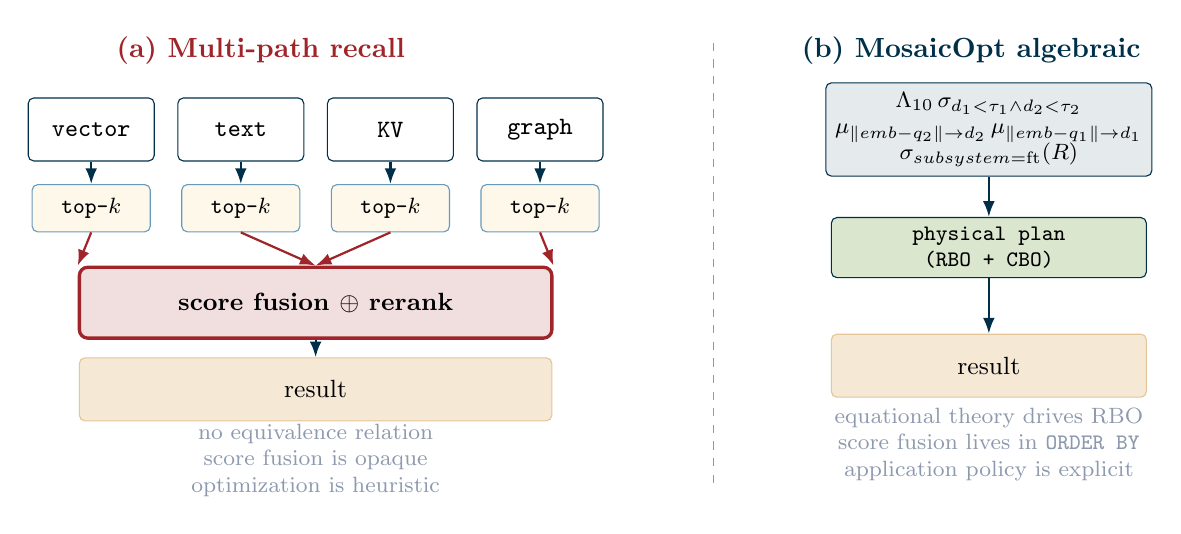
\begin{tikzpicture}[
    box/.style={rectangle, draw=mosaicBlue, fill=white, rounded corners=2pt, minimum height=0.8cm, font=\ttfamily\small, align=center},
    scorebox/.style={rectangle, draw=mosaicLightBlue, fill=mosaicCream!50, rounded corners=2pt, minimum height=0.6cm, font=\ttfamily\footnotesize, align=center},
    fusionbox/.style={rectangle, draw=mosaicCrimson, fill=mosaicCrimson!15, very thick, rounded corners=3pt, minimum height=0.9cm, font=\small\bfseries, align=center},
    planbox/.style={rectangle, draw=mosaicBlue, fill=white, rounded corners=2pt, minimum height=0.7cm, font=\ttfamily\footnotesize, align=center},
    resultbox/.style={rectangle, draw=mosaicTan, fill=mosaicTan!40, rounded corners=2pt, minimum height=0.8cm, font=\small, align=center},
    arr/.style={-{Latex[length=2mm]}, thick, color=mosaicBlue},
    arr2/.style={-{Latex[length=2mm]}, thick, color=mosaicCrimson}
  ]
    % Left side: Multi-path recall
    \node[font=\bfseries, color=mosaicCrimson, anchor=west] at (-7.2,3.2) {(a) Multi-path recall};
    \node[box, minimum width=1.6cm] (v1) at (-7.4,2.2) {vector};
    \node[box, minimum width=1.6cm] (t1) at (-5.5,2.2) {text};
    \node[box, minimum width=1.6cm] (k1) at (-3.6,2.2) {KV};
    \node[box, minimum width=1.6cm] (g1) at (-1.7,2.2) {graph};
    \node[scorebox, minimum width=1.5cm] (vs1) at (-7.4,1.2) {top-$k$};
    \node[scorebox, minimum width=1.5cm] (ts1) at (-5.5,1.2) {top-$k$};
    \node[scorebox, minimum width=1.5cm] (ks1) at (-3.6,1.2) {top-$k$};
    \node[scorebox, minimum width=1.5cm] (gs1) at (-1.7,1.2) {top-$k$};
    \node[fusionbox, minimum width=6.0cm] (fu) at (-4.55,0.0) {score fusion $\oplus$ rerank};
    \node[resultbox, minimum width=6.0cm] (res1) at (-4.55,-1.1) {result};
    \draw[arr] (v1) -- (vs1);
    \draw[arr] (t1) -- (ts1);
    \draw[arr] (k1) -- (ks1);
    \draw[arr] (g1) -- (gs1);
    \draw[arr2] (vs1.south) -- (fu.north west);
    \draw[arr2] (ts1.south) -- (fu.north);
    \draw[arr2] (ks1.south) -- (fu.north);
    \draw[arr2] (gs1.south) -- (fu.north east);
    \draw[arr] (fu) -- (res1);
    \node[font=\footnotesize, color=mosaicGray, align=center] at (-4.55,-2.0) {no equivalence relation \\ score fusion is opaque \\ optimization is heuristic};

    % Right side: MosaicOpt algebraic
    \node[font=\bfseries, color=mosaicBlue, anchor=west] at (1.5,3.2) {(b) MosaicOpt algebraic};
    \node[planbox, minimum width=4.0cm, fill=mosaicBlue!10] (log) at (4.0,2.2) {$\Lambda_{10}\,\sigma_{d_1<\tau_1\wedge d_2<\tau_2}$ \\ $\mu_{\lVert emb-q_2\rVert\to d_2}\,\mu_{\lVert emb-q_1\rVert\to d_1}$ \\ $\sigma_{subsystem=\mathrm{ft}}(R)$};
    \node[planbox, minimum width=4.0cm, fill=mosaicOlive!40] (cbo) at (4.0,0.7) {physical plan \\ \footnotesize (RBO + CBO)};
    \node[resultbox, minimum width=4.0cm] (res2) at (4.0,-0.8) {result};
    \draw[arr] (log) -- (cbo);
    \draw[arr] (cbo) -- (res2);
    \node[font=\footnotesize, color=mosaicGray, align=center] at (4.0,-1.8) {equational theory drives RBO \\ score fusion lives in \texttt{ORDER BY} \\ application policy is explicit};

    % Vertical separator
    \draw[dashed, color=mosaicGray] (0.5,3.3) -- (0.5,-2.3);
  \end{tikzpicture}%
  }
  \Description{Side-by-side comparison: (a) Multi-path recall with four parallel boxes (vector, text, KV, graph) feeding into four top-k score lists, then a fusion box (brick red), then result (warm tan); versus (b) MosaicOpt algebraic with one logical plan, one physical plan (olive), then result (warm tan).}
  \caption{Multi-path recall (a) vs. MosaicOpt algebraic (b).}
  \label{fig:multipath}
\end{figure}

Figure~\ref{fig:multipath} delineates two alternative architectures: (a) four independent channels are provided as inputs to a fusion component in the absence of any defined equivalence relation; (b) the user specifies a single logical plan, the RBO systematically enumerates equivalent rewrites under the governing equational theory, the CBO selects an appropriate physical implementation, and the fusion policy is made explicit via \texttt{ORDER BY}. This comparison is salient along three dimensions. First, \emph{equivalence}: configuration (a) lacks a formal notion of equivalence, whereas (b) is grounded in an explicit equational theory. Second, \emph{rewrites}: configuration (a) corresponds to a manually engineered orchestration pipeline, whereas (b) yields rewrites produced by the rule-based optimizer. Third, \emph{extension}: configuration (a) necessitates modifications to pipeline code whenever a new modality or fusion policy is introduced, whereas (b) requires only the addition of the corresponding operator and its algebraic identities to the underlying algebra.

\section{The Extended Algebra: Syntax \& Semantics}\label{sec:algebra}

We extend the classical relational algebra with four new constructs: a \emph{materialization} operator $\mu$ that lifts computed values (vector distances, BM25 scores, derived attributes) to first-class attributes; first-class multi-modal predicates
(vector range, BM25 relevance, graph reachability); $k$NN join over a pair of vectorized columns; and a \emph{graph expansion} operator $\Gamma$. Bag semantics apply throughout (matching SQL, avoiding row-collapse anomalies of set semantics with duplicate memory units). 

The full operator inventory:

\begin{table}[t]
  \centering
  \scriptsize
  \caption{Logical operators of the extended algebra. (In a table $R$, each attribute $A$, the entry of which should remain atomic logically, can be either scalar values, vectors, or texts.)}
  \label{tab:ops}
  \begin{tabular}{@{}p{2.0cm}p{2.6cm}p{3.1cm}@{}}
    \toprule
    Operator & Syntax & Meaning \\
    \midrule
    Materialization & $\mu_{e\to c}(R)$ & Per row, compute $e$; bind to $c$. \\
    Approximate Join & $R \bowtie_{distance(a,b)\le\tau} S$ & approximate join between $R$ and $S$. \\
    Graph expansion & $\Gamma_{g,d}(R)$ & From node-id, traverse $g$ to depth $d$. \\
    \bottomrule
  \end{tabular}
\end{table}

\paragraph{Graph modality as a first-class edge relation.}
The graph modality is realized through a \emph{distinguished first-class edge relation} $\KG(\mathit{src}, \mathit{dst}, \mathit{label})$ that lives in the schema alongside $\Mem$ and any other user-declared relations. $\Gamma$'s subscript $g$ in $\Gamma_{g,d}(L)$ is the \emph{edge label filter} on $\KG.label$, so $\Gamma_{\mathrm{derived\_from},\,d=1}(Q_4)$ means: take each row of $Q_4$ as an origin, walk $\KG$ restricted to edges with $\mathit{label}=\texttt{derived\_from}$, and return the rows reachable within one hop, joined with $Q_4$'s other attributes. $\Gamma$ does not need a second argument: the graph is a system-level resource like the base relation $\Mem$, and the subscript $g$ selects which edges within that resource to follow. The mapping from graph modality to the algebra is therefore one-to-one: $\Mem$ carries the memory-unit rows, $\KG$ carries the edges, and $\Gamma$ is the operator that closes the loop.

Existing semantics: a relation is a multiset; $\sigma$, $\mu$, $\Gamma$ preserve row multiplicity; $\cup$ adds, $\cap$ takes $\min$, $-$ subtracts; $\tau_o$ orders (subscript $o$ names the sort column list, \eg $\tau_{d_1,d_2}$ sorts by $(d_1,d_2)$); $\Lambda_k$ truncates (subscript $k$ is the row count, \eg $\Lambda_{10}$ keeps the top $10$); $\Gamma_g$ expands $\KG$ along edges of label $g$.

A predicate $\varphi$ is a Boolean combination of atoms over the input attributes: \emph{classical} ($A = c$, $A < c$, $A \in S$). We extend it by enabling the predicate to involve vector distance, text similarity, and graph reachability tests, \ie $\lVert V_a - q\rVert < \tau$ for query-time bound $q$, threshold $\tau$, $\mathrm{BM25}(t, q) > \theta$, and $\mathrm{reachable}(u, v)$, $\mathrm{edge}(u, v, \ell)$. Specifically, we list the newly introduced predicates as follows,
\begin{itemize}
    \item \emph{vector}: $\lVert V_a - q\rVert < \tau$, where $V_a$ is a vector-valued attribute, $q$ is a query-time bound parameter, and $\tau \geq 0$ is a distance threshold; equality and other comparison operators are admissible, range ($< \tau$) is the most important form;
    \item \emph{text}: $\texttt{BM25}(t, q) > \theta$, where $t$ is a text attribute, $q$ a query-time bound string, and $\theta$ a relevance threshold; we use Okapi BM25 with parameters $(k_1, b)$ carried with the predicate;
    \item \emph{graph}: $\texttt{reachable}(u, v)$ boolean and $\texttt{edge}(u, v, \ell)$
for nodes $u, v$ in a graph attribute, $\ell$ a label or wildcard.
\end{itemize}
The query-time bound parameters ($q$, $\tau$, $\theta$) are first-class values supplied at execution time, distinct from input attributes: they make predicates safely late-binding. The algebra expression is the same across query instances; only the bound  parameters change.

A materialization expression \(e\) is evaluated per tuple. Supported forms include: (i) scalar expressions (\eg \(A+B\), \(f(A)\)); (ii) vector expressions (\eg \(\lVert V_a-q\rVert\)); (iii) text-retrieval expressions (\eg \(\texttt{BM25}(t,q)\)); (iv) Boolean/arithmetic compositions of the above; and (v) constants \(\mathrm{true}\), \(\mathrm{false}\), and \(\mathrm{null}\). The expression language is intentionally limited to user-visible SQL/MM-style predicates and to forms with estimable costs in the model.

The key property of \(\mu\) is that it promotes the computed value to a first-class output attribute. After materialization, the value can be referenced by downstream selection \(\sigma\), projection \(\pi\), \texttt{ORDER BY} within sorting \(\tau\), and later \(\mu\) expressions. This lets the system expose per-column distances to application \texttt{ORDER BY} semantics without dropping them during execution.

In \(\mu_{e\to c}(L)\), the requirement that \(c\) be fresh (\ie absent from the input schema) functions as a hygienic condition to avoid name capture, rather than constituting a semantic constraint. When necessary, a renaming operation \(\rho\) may be applied to generate an appropriate fresh identifier.

The denotational semantics of the \(\mu\) operator is given by the multiset \(\{\, r \oplus \{c \mapsto e(r)\} : r \in R \,\}\), where \(\oplus\) extends each tuple \(r\) with a binding that assigns the fresh attribute \(c\) the value obtained by evaluating \(e\) on \(r\). If \(e(r)\) is undefined (\eg when computing a distance to a null vector), the corresponding tuple is omitted from the result. This behavior is consistent with SQL \texttt{NULL}-propagation conventions and is required to ensure safety in the presence of missing embeddings.

\paragraph{Why not the classical assignment/extend operator?}
The extended-relational-algebra literature has long offered an \emph{assignment} or \emph{extend} operator, \ie $R.a := E$ or $R \oplus \{a \mapsto E\}$, that re-binds (or extends) one attribute of $R$ in place~\cite{abiteboul1995foundations}. $\mu$ differs in a single, decisive way: it is the optimizer's \emph{first-class surface} for per-row multi-modal evaluation. The per-row expression $e$, the named binding $c$, the cost dimension $T_\mu$ (per-row evaluation cost, HNSW-bound for vector distances), and the M1--M5 redex patterns are all anchored on the $\mu$ node type. Two examples make the difference concrete. \emph{(i)~Cost pricing.} Take $Q = \sigma_{d<\tau}\bigl(\mu_{\lVert\mathit{emb}-q\rVert\to d}(R)\bigr)$ with $n = |R| = 10^4$, $d = 128$, and selectivity $s \approx 10^{-3}$. With $\mu$, the cost model sees a $\mu$ node and prices it as an ANN-bound $T_\mu \approx 0.5\,\mathrm{ms}$ (HNSW \texttt{efSearch}$=64$), so the CBO correctly picks HNSW. An equivalent plan written as $\sigma_{d<\tau}\bigl(\pi_{\dots, \lVert\mathit{emb}-q\rVert}(R)\bigr)$ exposes only a generic projection node, and the cost model prices $T_\pi$ an order of magnitude lower, so the CBO wrongly picks a flat scan. \emph{(ii)~Rewriter anchoring.} The RBO's M1 redex $\sigma_{c<\tau} \circ \mu_{e \to c}$ is anchored on a $\mu$ node; rewriting it to $\mu_{e \to c} \circ \sigma_{e < \tau}$ saves a $(1-s)\cdot n$ factor of per-row distance computation. With a $\pi$-based encoding, M1 has no node type to match and does not fire, so the distance is computed for every row regardless of selectivity---at $s = 10^{-3}$, that is a $1000\times$ wasted work. Classical assignment is a general-purpose extension that is not anchored on a rewriter or a cost entry; the multi-modal workload would lose both.

The approximate join operator, $R \bowtie_{dist(a,b)\le\tau} S$, performs a $\theta$ join over $R$ and $S$, where $\theta$ is extended to involve distance filters over vectors and text columns. Specifically, for each tuple in $R$, it joins with those tuples in $S$ whose entries in column $S.b$ are within (or beyond) the distance predicate $\tau$, with respect to the entry of $R.a$. Hereby, the distance (\(dist(a,b)\)) can be either \(\texttt{BM25}(a,b)\) or \(||a-b||\).

\paragraph{When is this operator forced?}
The "approximate" qualifier in the operator's name refers to the \emph{physical} implementation, not the logical semantics: the logical operator computes the exact $\theta$-join on the distance predicate, but the cost model admits an ANN-backed physical realization (an HNSW traversal of the inner relation) since the cross-table $\theta$-join over a distance threshold has no classical B-tree acceleration. This operator is forced by three workload shapes for which no other relational construct suffices. \emph{(i)~Cross-table semantic join}, \eg "find \texttt{Passages} with description similar to \texttt{Incidents.description}", joining two relations that share no key; classical equi-join infrastructure does not apply, and a nested-loop $\mu$ over the inner relation is asymptotically worse than the ANN-walked join this operator licenses. \emph{(ii)~Near-duplicate detection}, $R \bowtie_{\lVert a-b\rVert \le \tau} R$, the canonical de-duplication pattern where the join key is a vector distance. \emph{(iii)~Entity matching over heterogeneous embeddings}, joining users to sessions by content vector similarity when the two sides are not even in the same relation schema. In all three cases the join key is a vector (or BM25) distance, so the operator exists exactly to give that pattern a first-class place in the algebra.

\textbf{Running example.} Let $\Mem$ be a memory-unit relation with attributes $\mathit{id}$, $\mathit{text}$, $\mathit{ts}$, $\vect{emb}$, $\vect{emb\_alt}$, $\mathit{user}$, $\mathit{subsystem}$, and let $\KG(\mathit{src}, \mathit{dst}, \mathit{label})$ hold derivation links. The query ``semantically similar passages in the
fault-tolerance subsystem from the last 30 days, top 10 by $(d_1, d_2)$'' is:
\begin{align*}
Q_1 &= \Mem \\
Q_2 &= \sigma_{\mathit{subsystem}=\mathrm{ft} \wedge
         \mathit{ts} > \mathrm{now}-30d}(Q_1) \\
Q_3 &= \mu_{\lVert\vect{emb}-\vect{q}_1\rVert\to d_1}\;
        \mu_{\lVert\vect{emb\_alt}-\vect{q}_2\rVert\to d_2}(Q_2) \\
Q_4 &= \sigma_{d_1<\tau_1 \wedge d_2<\tau_2}(Q_3) \\
Q_5 &= \Lambda_{10}(\tau_{d_1,d_2}(Q_4))
\end{align*}


\begin{figure}[t]
  \centering
  \resizebox{\columnwidth}{!}{%
  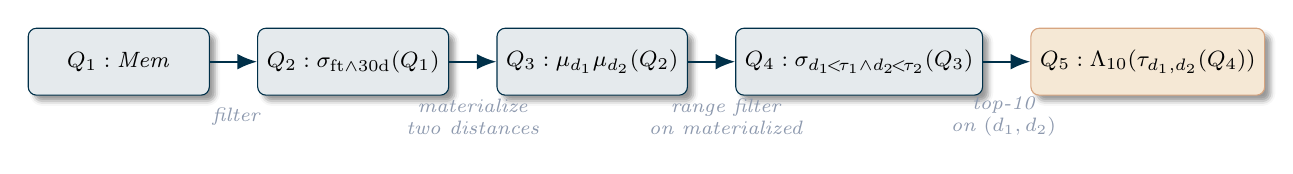
\begin{tikzpicture}[
    qbox/.style={rectangle, draw=mosaicBlue, fill=mosaicBlue!10, rounded corners=3pt, minimum width=2.3cm, minimum height=0.85cm, font=\ttfamily\footnotesize, align=center, blur shadow={shadow blur steps=3}},
    finalbox/.style={rectangle, draw=mosaicTan!80!mosaicCrimson, fill=mosaicTan!40, rounded corners=3pt, minimum width=2.3cm, minimum height=0.85cm, font=\ttfamily\footnotesize, align=center, blur shadow={shadow blur steps=3}},
    ann/.style={font=\scriptsize\itshape, color=mosaicGray, align=center},
    arr/.style={-{Latex[length=2.5mm,width=2mm]}, thick, color=mosaicBlue}
  ]
    \node[qbox] (q1) at (0,0) {$Q_1: \Mem$};
    \node[qbox, right=0.6cm of q1] (q2) {$Q_2: \sigma_{\mathrm{ft}\wedge\mathrm{30d}}(Q_1)$};
    \node[qbox, right=0.6cm of q2] (q3) {$Q_3: \mu_{d_1}\mu_{d_2}(Q_2)$};
    \node[qbox, right=0.6cm of q3] (q4) {$Q_4: \sigma_{d_1\!<\!\tau_1\wedge d_2\!<\!\tau_2}(Q_3)$};
    \node[finalbox, right=0.6cm of q4] (q5) {$Q_5: \Lambda_{10}(\tau_{d_1,d_2}(Q_4))$};
    \draw[arr] (q1) -- (q2);
    \draw[arr] (q2) -- (q3);
    \draw[arr] (q3) -- (q4);
    \draw[arr] (q4) -- (q5);

    % Annotations under the arrows
    \node[ann] at ($(q1)!0.5!(q2) + (0,-0.7)$) {filter};
    \node[ann] at ($(q2)!0.5!(q3) + (0,-0.7)$) {materialize\\two distances};
    \node[ann] at ($(q3)!0.5!(q4) + (0,-0.7)$) {range filter\\on materialized};
    \node[ann] at ($(q4)!0.5!(q5) + (0,-0.7)$) {top-10\\on $(d_1,d_2)$};
  \end{tikzpicture}%
  }
  \Description{Horizontal pipeline with five boxes: Q1 (base relation Mem), Q2 (filter on subsystem and timestamp), Q3 (materialize two distances), Q4 (range filter), Q5 (top-10 on the materialised distance columns $(d_1, d_2)$, terminal box highlighted in warm tan). Arrows between boxes show data flow.}
  \caption{The running example $Q_1 \to Q_5$ as a horizontal pipeline; the warm-tan terminal box is the top-$K$ over the materialised distance columns.}
  \label{fig:pipeline}
\end{figure}

Figure~\ref{fig:pipeline} shows the same example as a horizontal pipeline. Each box is a logical operation, emphasizing compositionality: each $Q_i$ can be referenced as input to the next stage.

A graph-aware variant (\ie ``the same computation, restricted to memories connected via a \texttt{derived\_from} chain to a known incident''? can be formalized as
\begin{align*}
R_1 &= \sigma_{\mathit{id} = 42}(\Mem) &&\text{--- the seed incident} \\
R_2 &= \Gamma_{\mathrm{derived\_from},\,d=2}(R_1) &&\text{--- two hops downstream} \\
R_3 &= \sigma_{\mathit{id} \in \pi_{\mathit{dst}}(R_2)}(Q_2) &&\text{--- intersect with filter}
\end{align*}
followed by the same $\mu$/$\sigma$/$\tau$/$\Lambda$ sequence. Here, $\Gamma$ composes with the rest of the algebra. This example shows that (i) the algebra is closed under composition (each operator outputs a logical plan usable as input to any other operator); and (ii) graph expansion composes with the algebra like selection, projection, and join.
\section{Equational Theory: Identities and Non-Identities}\label{sec:equational}

\subsection{Why these operators?}

Why $\sigma$, $\pi$, $\cup$, $-$, $\rho$, $\times$, $\tau$, $\Lambda$?
They are the classical relational algebra; we do not add or remove
any of them. Why $\mu$ (materialization) and $\Gamma$ (graph
expansion)? They are the two operators needed to express the
Agentic-memory workload in the algebraic form, every
memory query either materializes a computed value (a distance,
a relevance score, a derived attribute) or expands the graph
(traverses a derivation chain). The fusion pattern
$\mu_{d_a}\,\mu_{d_b}\,\sigma_{d_a<\tau_a\wedge d_b<\tau_b}\,
\tau_{d_a + d_b}\,\Lambda_k$ from Section~\ref{sec:algebra}
is the canonical multi-modal fusion; the
$\sigma_{\varphi}\,\mu_{e\to c}\,\Gamma_{g,d}$ chain is
the canonical graph-aware materialization. The choice of these
two operators is the minimum that makes the Agentic-memory
workload expressible; adding more operators would only
complicate the rewrite theory without expanding the
expressive power. Operators we did \emph{not} add: a path
operator (expressible as $\mu$ + $\Gamma$), a streaming
operator (orthogonal to the algebra), a probabilistic
operator (future work, see Section~\ref{sec:discuss:open}).

The optimizer (Section~\ref{sec:rbo}) is driven by an
\emph{equational theory}: a set of identities over logical plans.
The same theory also records, explicitly, the identities that
classical intuition suggests but approximation breaks, the
\emph{non-identities}, so the optimizer knows not to apply them.
This section unifies both sides. We first give an overview
(4.1), then the inherited classical axioms (4.2), then the new
identities that the extended operators license (4.3), then the
derived rewrites the optimizer uses (4.4), and finally the
non-identities with counterexamples (4.5).

\subsection{Overview}\label{sec:equational:overview}

The equational theory of the extended algebra plays two
complementary roles. \emph{First}, it is the foundation for the
rule-based optimizer (Section~\ref{sec:rbo}): every rewrite the
RBO performs is justified by a foundational identity (M1--M5, G1,
G2) or by a derived corollary / definitional / implied rule (A4-vector,
A4-vector+M1, M4+M1, M5+G1, A7-symmetry, A8-regroup, $\topK$
recognition, $\sigma$-$\tau$ commutation), so the optimizer's
behaviour is auditable, not opaque. \emph{Second}, the
\emph{non}-identities (N1--N5) are the discipline that prevents
the optimizer from applying rewrites that hold in classical
relational algebra but break under approximation, graph-traversal
asymmetry, or the traversal-vs-origin column split. The cost model
(Section~\ref{sec:cbo}) is responsible for the physical cost of
every rewrite; the equational theory is responsible for its
\emph{correctness}.

Concretely, an identity is an equation of the form
\texttt{LHS = RHS} between two logical plans that hold for all
instances of the free variables (relation names, attribute names,
query-time bound parameters). A non-identity is a pair of plans
that classical intuition might equate but the extended setting
does not, with an explicit counterexample. Both are first-class
objects: the RBO loads them as data, the cost model consults them
when computing the ``cost of identity application'' term, and the
executor relies on them for safety of adaptive re-planning
(Section~\ref{sec:cbo}).

The structure of this section follows the algebra's structure:
inherited axioms (the ones we use but do not re-prove) in
Section~\ref{sec:equational:inherited}; new identities (the ones
the extended operators license) in
Section~\ref{sec:equational:new}; derived rules (combinations used
directly by the optimizer) in
Section~\ref{sec:equational:derived}; and non-identities
(counterexamples that bound the optimization horizon) in
Section~\ref{sec:equational:nonident}.

\subsection{Inherited foundational axioms}\label{sec:equational:inherited}

The following four identities are the assumed classical axioms the
new rules actually depend on. Each is named because the
rewriter in Section~\ref{sec:rbo} matches it explicitly. Other
standard classical identities (selection over union, projection
idempotence, projection--join pushdown, rename involutivity, etc.)
hold throughout the paper and are taken as implicitly assumed; we
omit them because no rule in the new equational theory anchors on
them.\footnote{Concretely, A2, A3, A5, A6 are not referenced by any
identity M1--M6, G1--G3, or by the rewrites they license. They are
standard textbook axioms and are part of the implicit closed-world
assumption on the classical algebra.}

\begin{itemize}[leftmargin=*]
  \item \textbf{(A1) Selection composition.}
    $\sigma_\varphi \sigma_\psi(L) = \sigma_{\varphi \wedge \psi}(L)$.
    Used by the rewriter to split a conjunctive $\sigma$ into
    per-predicate selections, so each can be pushed individually
    (see M1, M6, A4-vector, V1).
  \item \textbf{(A4) Selection--join pushdown.} If every attribute
    mentioned in $\varphi$ is in the schema of $L$, then
    $\sigma_\varphi(L \bowtie_\psi M) = \sigma_\varphi(L) \bowtie_\psi M$.
    Used by the rewriter to push predicates that reference only one
    side of a join (M4 and its corollary A4-vector).
  \item \textbf{(A7) Join commutativity.} For any symmetric
    predicate $\psi$, $L \bowtie_\psi M = M \bowtie_{\psi^{\mathrm{sym}}} L$.
    The two sides are identical as multisets; the cost is not
    (Theorem~\ref{thm:n2}). The RBO generates both LHS and RHS
    orderings; the CBO picks the cheaper side.
  \item \textbf{(A8) Join associativity.} For independent
    predicates $\psi$, $\chi$ with no attribute ambiguity,
    $L \bowtie_\psi (M \bowtie_\chi N) = (L \bowtie_\psi M) \bowtie_\chi N$.
    This is the identity the RBO uses to enumerate the $O(n!)$
    join orderings.
\end{itemize}

These hold for any predicate in our extended form (classical,
vector, text, graph) provided the attribute references are
respected. We do not claim any new identities here; we merely
note that the extended predicates do not violate them.

\subsection{New foundational axioms}\label{sec:equational:new}

We introduce the \emph{nine} identities that the extended algebra
makes possible. Each is stated in a form that names the conditions
for its applicability. (Two further rules, \textbf{V1} and
\textbf{J1}, are corollaries of the assumed classical axioms
A1 and A4 with vector-predicate specialization; they are kept as
named redex patterns in the RBO code but have no separate theorem
block. The $\tau$-$\Lambda$-$\topK$ family and the
$\sigma$-$\tau$ commutation are \emph{implied} by the operator
definitions: $\topK_O(L, K):= \tau_o(\Lambda_k(L))$ from
Section~\ref{sec:algebra} and the row-preserving semantics of
$\sigma$ and $\tau$. The RBO uses them as zero-weight rewrites in
the ARS, but they have no separate theorem block.)

Each identity below is followed by a brief \emph{cost-effect
annotation} that names the optimization the rewrite enables; the
RBO fires the rewrite as part of its greedy loop
(Section~\ref{sec:rbo:role}).

\begin{theorem}[M1: Selection commutes with materialization on the materialized column]\label{thm:m1}
Where $c$ is a fresh attribute name and $e$ is an expression
depending only on attributes of $L$:
\[
\sigma_{c < \tau}\, \mu_{e \to c}(L) \;=\; \mu_{e \to c}\, \sigma_{e < \tau}(L).
\]
\end{theorem}

  (Proof in Appendix~\ref{app:proofs}.)

\begin{figure}[t]
  \centering
  \resizebox{\columnwidth}{!}{%
  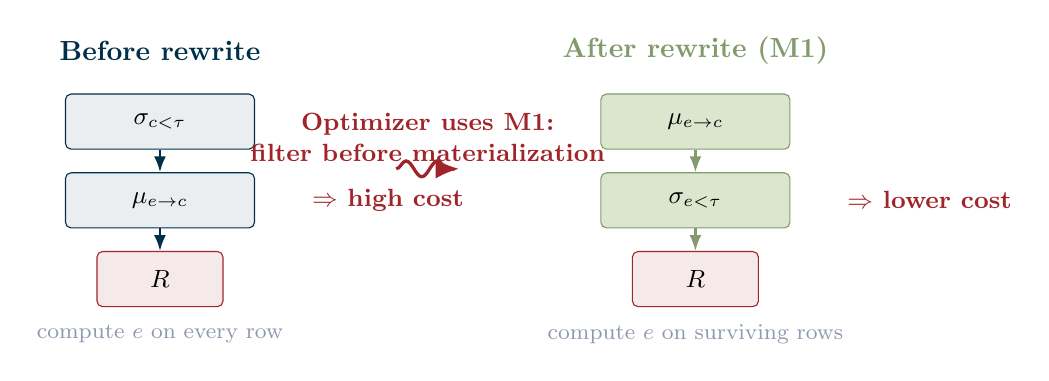
\begin{tikzpicture}[
    node distance=0.4cm and 0.6cm,
    op/.style={rectangle, draw=mosaicBlue, fill=mosaicBlue!8, rounded corners=2pt, minimum width=2.4cm, minimum height=0.7cm, font=\ttfamily\small, align=center},
    rnode/.style={rectangle, draw=mosaicCrimson, fill=mosaicCrimson!10, rounded corners=2pt, minimum width=1.6cm, minimum height=0.7cm, font=\ttfamily\small, align=center},
    op2/.style={rectangle, draw=mosaicOlive!80!black, fill=mosaicOlive!40, rounded corners=2pt, minimum width=2.4cm, minimum height=0.7cm, font=\ttfamily\small, align=center},
    arr/.style={-{Latex[length=2mm]}, thick, color=mosaicBlue},
    arr2/.style={-{Latex[length=2mm]}, thick, color=mosaicOlive!80!black},
    ann/.style={font=\footnotesize, color=mosaicGray, align=center},
    cost/.style={font=\small\bfseries, color=mosaicCrimson}
  ]
    % Left tree (before rewrite)
    \node[font=\bfseries, color=mosaicBlue] at (-3.4, 2.4) {Before rewrite};
    \node[op] (leftsigma) at (-3.4, 1.5) {$\sigma_{c<\tau}$};
    \node[op] (leftmu) at (-3.4, 0.5) {$\mu_{e\to c}$};
    \node[rnode] (leftR) at (-3.4, -0.5) {$R$};
    \draw[arr] (leftsigma) -- (leftmu);
    \draw[arr] (leftmu) -- (leftR);
    \node[ann, below=0.1cm of leftR] {compute $e$ on every row};
    \node[cost, right=0.0cm of leftmu, xshift=0.6cm] {$\Rightarrow$ high cost};

    % Right tree (after rewrite) -- olive green for the optimized outcome
    \node[font=\bfseries, color=mosaicOlive!80!black] at (3.4, 2.4) {After rewrite (M1)};
    \node[op2] (rightmu) at (3.4, 1.5) {$\mu_{e\to c}$};
    \node[op2] (rightsigma) at (3.4, 0.5) {$\sigma_{e<\tau}$};
    \node[rnode] (rightR) at (3.4, -0.5) {$R$};
    \draw[arr2] (rightmu) -- (rightsigma);
    \draw[arr2] (rightsigma) -- (rightR);
    \node[ann, below=0.1cm of rightR] {compute $e$ on surviving rows};
    \node[cost, right=0.0cm of rightsigma, xshift=0.6cm] {$\Rightarrow$ lower cost};

    % Optimization arrow
    \draw[-{Latex[length=3mm,width=2.5mm]}, very thick, color=mosaicCrimson, decorate, decoration={snake, amplitude=1mm, segment length=4mm}] (-0.4,0.9) -- (0.4,0.9);
    \node[ann, color=mosaicCrimson, font=\small\bfseries] at (0,1.3) {Optimizer uses M1:\\filter before materialization};
  \end{tikzpicture}%
  }
  \Description{Two tree diagrams side by side. Left (before rewrite, blue): $\sigma_{c<\tau}$ on top of $\mu_{e\to c}(R)$ -- both $e$ computation and filtering happen. Right (after rewrite, olive): $\mu_{e\to c}$ on top of $\sigma_{e<\tau}(R)$ -- filter first, then compute. Annotation: cost saving is that $e$ is computed only on rows that survive the filter.}
  \caption{Visualization of the M1 rewrite: the optimizer swaps $\sigma$ and $\mu$ so that $e$ is computed only on rows that survive the filter. The optimized side is rendered in the soft-olive accent to make the rewrite visible at a glance.}
  \label{fig:m1}
\end{figure}

Figure~\ref{fig:m1} visualizes the M1 rewrite. The \emph{left} tree
shows the input plan: $\sigma_{c<\tau}$ on top of $\mu_{e\to c}(R)$,
which materializes $e$ on every row and then filters on $c < \tau$.
The \emph{right} tree shows the rewritten plan: $\mu_{e\to c}$ on
top of $\sigma_{e<\tau}(R)$, which applies the filter
\emph{before} materialization; $e$ is computed only on rows that
survive the filter. The cost saving scales with the selectivity
of $e < \tau$, for a tight vector range the selectivity can be
one part in $10^3$ or smaller, and the saving is correspondingly
dramatic.

\begin{theorem}[M2: Materialization is commutative]\label{thm:m2}
For fresh names $c_1, c_2$ and expressions $e_1, e_2$ depending
only on $L$'s attributes (and not on each other's outputs):
\[
\mu_{e_1 \to c_1}\, \mu_{e_2 \to c_2}(L)
\;=\;
\mu_{e_2 \to c_2}\, \mu_{e_1 \to c_1}(L).
\]
\end{theorem}

  (Proof in Appendix~\ref{app:proofs}.)

\begin{theorem}[M3: Materialization through projection]\label{thm:m3}
For fresh $c$ and expression $e$ depending only on attributes in $A$:
\[
\mu_{e \to c}\, \pi_A(L) \;=\; \pi_{A \cup \{c\}}\, \mu_{e \to c}(L).
\]
\end{theorem}

  (Proof in Appendix~\ref{app:proofs}.)

\begin{theorem}[M4: Materialization pushdown through join]\label{thm:m4}
Where $e$ depends only on attributes of $L$ and $c$ is a fresh
attribute name:
\[
\mu_{e \to c}\, (L \bowtie_\psi M)
\;=\;
(\mu_{e \to c}(L)) \bowtie_\psi M.
\]
\end{theorem}

  (Proof in Appendix~\ref{app:proofs}.)

\begin{theorem}[M5: Materialization pushdown through graph expansion]\label{thm:m5}
Where $e$ depends only on attributes of $L$, $c$ is fresh, and $c$
is not the graph rule's node-id attribute:
\[
\mu_{e \to c}\, \Gamma_{g, d}(L)
\;=\;
\Gamma_{g, d}\, \mu_{e \to c}(L).
\]
This is the $\mu$-counterpart of G1 and the rewrite the RBO
generates for graph queries that materialize a per-origin attribute
(e.g.\ a distance to a fixed query point) and then expand. The
two sides produce the same multiset of $(r, v, c)$ tuples; the
cost differs because the LHS computes $e$ on every traversal row
while the RHS computes $e$ on every origin row. When
$|\Gamma_{g,d}(L)| > |L|$ (the typical case for $d \geq 1$ and a
non-trivial graph), the RHS is cheaper, and the CBO picks it.
\end{theorem}

  (Proof in Appendix~\ref{app:proofs}.)

\begin{theorem}[M6: Selection on input attributes commutes with materialization]\label{thm:m6}
Where $\varphi$ references only attributes of $L$ (and not the
fresh attribute $c$):
\[
\sigma_\varphi\, \mu_{e \to c}(L)
\;=\;
\mu_{e \to c}\, \sigma_\varphi(L).
\]
\emph{Cost effect:} the LHS computes $e$ on every row of $L$ and
then filters; the RHS filters first and computes $e$ only on the
$s$-fraction that survives. For selectivity $s$, the saving is
$(1-s) \cdot |L| \cdot T_\mu$ per-row evaluations. M6 is the
classical-filter complement of M1: M1 handles
$\sigma_{c<\tau} \circ \mu_{e \to c}$ (predicates that reference
$c$, the materialised attribute); M6 handles
$\sigma_\varphi \circ \mu_{e \to c}$ (predicates that reference
only the input schema, the typical case for
$\sigma_{\mathit{subsys}=\mathrm{known}} \circ \mu$ in the running
example). Together they cover every $\sigma$--$\mu$ redex.
\end{theorem}

  (Proof in Appendix~\ref{app:proofs}.)

\begin{theorem}[G1: Selection pushdown through graph expansion]\label{thm:g1}
Where $\varphi$ references only attributes of $L$ (and not
attributes of the graph rule's traversal result):
\[
\sigma_\varphi\, \Gamma_{g, d}(L) \;=\; \Gamma_{g, d}\, \sigma_\varphi(L).
\]
\end{theorem}

  (Proof in Appendix~\ref{app:proofs}.)

\begin{theorem}[G2: Graph expansion is transitive]\label{thm:g2}
Let $g_1, g_2$ be graph rules over the same graph attribute
with disjoint label sets. If $g_1$'s traversal-result
attribute and $g_2$'s source attribute are disjoint (no
intermediate node of $g_2$ is a valid origin of $g_1$),
then the composition $g_1; g_2$ satisfies:
\[
\Gamma_{g_1, d_1}\, \Gamma_{g_2, d_2}(L) \;=\;
\Gamma_{g_1;g_2,\, d_1+d_2}(L).
\]
\emph{Cost effect:} the LHS performs two graph walks (one of
depth $d_1$, one of depth $d_2$, each visiting a separate
frontier set of nodes) and materializes their intermediate
result; the RHS performs a single walk of depth $d_1 + d_2$
through the composite rule. For a graph with branching factor
$b$, the LHS visits $\sum_{i=0}^{d_1} b^i \cdot b^{d_2}$ nodes
across both walks (with intermediate expansion materialization
in between), while the RHS visits $\sum_{i=0}^{d_1+d_2} b^i$ nodes
in a single walk. G2 lets the RBO collapse nested
$\Gamma$s into a single expansion at depth $d_1 + d_2$
``two \texttt{derived\_from} hops'' becomes ``one
\texttt{derived\_from}; \texttt{derived\_from} hop''.
\end{theorem}

  (Proof in Appendix~\ref{app:proofs}.)

The G2 collapse is bounded by the number of nested-$\Gamma$
inversions in $P$ (one collapse per nesting, hence the depth $d$
of the result). G2 is a zero-weight rewrite: it does not change
the logical multiset, only the structure of the graph walk.

\begin{theorem}[G3: Projection pushdown through graph expansion]\label{thm:g3}
Let $A$ be an attribute set. Where $A$ does not include any
attribute introduced by $\Gamma$'s traversal step, and
$A' = A \cap \attr{L}$:
\[
\pi_A\, \Gamma_{g, d}(L)
\;=\;
\Gamma_{g, d}\, \pi_{A'}(L).
\]
\emph{Cost effect:} the LHS projects after expansion (every
traversal row carries the full schema), the RHS projects before
expansion (only the origin's narrower schema is carried through
the walk). G3 is the graph-expansion analog of A5
(projection--join pushdown). It is a zero-weight rewrite: plan
tree size is unchanged, but the row size at the $\Gamma$ input
is reduced, and on graphs with non-trivial branching the
saving compounds by the branching factor $b^d$.
\end{theorem}

  (Proof in Appendix~\ref{app:proofs}.)

\subsection{Derived identities}\label{sec:equational:derived}

By composing the foundational axioms and the assumed classical
identities, additional rewrites become available. The optimizer
uses these directly; we list them as corollaries rather than as
standalone foundational theorems to keep
Section~\ref{sec:equational:new} focused on the genuinely new
content.

\begin{itemize}[leftmargin=*]
  \item \textbf{A4-vector (in code: \texttt{J1}).} A4 specialized
    to a vector predicate:
    $\sigma_{\lVert V_a - q \rVert < \tau}\,(L \bowtie_\psi M) =
    (\sigma_{\lVert V_a - q \rVert < \tau}(L)) \bowtie_\psi M$
    when $V_a \in \attr{L}$, is what the CBO applies on the
    conjunctive multi-vector case. A1 likewise specializes to
    two vector predicates on distinct columns; the codebase
    calls this \texttt{V1}. Neither is a new algebraic identity,
    both follow from A1/A4 by predicate substitution: the
    codebase keeps them as named redex patterns (\texttt{V1},
    \texttt{J1}) so the RBO can match them explicitly without
    re-implementing A1/A4.
  \item \textbf{A7-symmetry (single application of A7).}
    Applying the assumed classical A7 in the reverse direction
    is a derived rewrite the RBO generates; the CBO then chooses
    the cheaper side per Theorem~\ref{thm:n2}.
  \item \textbf{A8-regrouping (single application of A8).}
    Applying the assumed classical A8 is the rewrite that exposes
    a different join parenthesization; the RBO uses it to
    enumerate the $O(n!)$ join orderings the CBO picks from.
  \item \textbf{$\topK$ recognition (definitional).} The
    abbreviation $\topK_O(L, K):= \tau_o(\Lambda_k(L))$ from
    Section~\ref{sec:algebra} makes
    $\tau_o\,\Lambda_k \leftrightarrow \topK_O$ a definitional
    rewrite; the CBO applies it as a physical-realization choice
    rather than as a logical RBO rewrite.
  \item \textbf{$\sigma$-$\tau$ commutation.} Trivially
    $\sigma_\varphi\,\tau_o(L) = \tau_o\,\sigma_\varphi(L)$
    (both operators are row-preserving). The RBO applies it as a
    zero-weight reordering, letting the CBO pick filter-first
    (avoids a full sort) or sort-first (enables top-$K$ early
    termination) by selectivity.
\end{itemize}

The nine foundational axioms, the four assumed classical identities
(A1, A4, A7, A8), the five derived / definitional rewrites above
(A4-vector/J1, A7-symmetry, A8-regrouping, T1, $\sigma$-$\tau$),
plus the rewrites that the rewriter composes on the fly (M4 then
M1, M5 then G1, M1 then A4-vector) together suffice to cover
the optimization of all plans whose operators draw from the
inventory of Section~\ref{sec:algebra}. The composed rewrites
(M4+M1, M5+G1, A4-vector+M1) are not new identities: each is
the application of two or more axioms in a fixed order. They are
recorded here as \emph{rewriter patterns} so the RBO can match
them as named templates (cf.\ Section~\ref{sec:rbo:trace}), but
they derive from the foundational identities above and are not
counted in the equational theory. Schema rules ensure that any
attribute a downstream operator references is either in the
input or has been introduced by a $\mu$. The identities are the
load-bearing ones for the Agentic-memory workload:

\begin{itemize}[leftmargin=*, itemsep=0pt]
  \item \textbf{M1} is the rewrite that makes vector-range
    queries cheap: it computes each distance only on rows that
    survive the filter, rather than on all $n$ rows. The
    cost-effect is $\sim (1 - s) \cdot n \cdot T_\mu$ work saved,
    where $s$ is the selectivity of the predicate being pushed
    and $T_\mu$ is the per-row cost of the materialization.
  \item \textbf{M6} is the classical-filter complement of M1:
    when the $\sigma$ predicate references only the input schema
    (not the materialised attribute $c$), the filter can be
    pushed below the materialization. This is the rewrite that
    makes the running example's
    $\sigma_{\mathit{subsys}=\mathrm{known}}$ fire before
    $\mu_{\Vert\mathit{emb}-q\Vert\to d}$: the subsystem check
    runs once, the vector distance is computed only on
    surviving rows.
  \item \textbf{M4, M5} extend materialization across joins and
    graph expansions so the same per-row computation is not
    repeated for every joined or expanded row. M4 is the
    join-side analogue of M1; M5 is the graph-side analogue. The
    cost-effect is the same as M1: $1 - s$ factor saving when
    the join/expansion has selectivity $s$. The rewrites
    ``M4 then M1'' and ``M5 then G1'' (composed in sequence by
    the RBO) chain the two rewriters for compound predicates.
  \item \textbf{G1} pushes selections through graph expansion
    when the predicate references only origin attributes. The
    cost-effect: the post-expansion row count is $\sim 1 - s$
    smaller, so the per-row work downstream of the expansion
    drops by the same factor. G1 fails on traversal attributes
    (N4), so the RBO must verify the compatibility check.
  \item \textbf{G2} collapses nested $\Gamma$s into a single
    walk of combined depth, removing the intermediate expansion
    materialization. This is a one-shot rewrite; it strictly
    decreases the structural weight.
  \item \textbf{G3} pushes projections above $\Gamma$ to below
    (analog of A5 for graph expansion). Cost-effect: the
    schema carried through the graph walk is narrowed before the
    walk, so each traversal row is smaller; on graphs with
    non-trivial branching the saving compounds by the branching
    factor. G3 is a zero-weight rewrite.
  \item The composed \emph{rewriter patterns}
    (\textbf{M4\,then\,M1}, \textbf{M5\,then\,G1},
    \textbf{M1\,then\,A4-vector}) are the dominant CBO wins on
    Q7 MV. Each is a sequence of two identity applications
    (see the bullet above on composed rewrites); the cost-effect
    is multiplicative: $(1-s_1) \cdot (1-s_2)$ of the work is
    saved.
  \item \textbf{T1} is the definitional $\tau\Lambda \to \topK$
    rewrite; modest at $n = 10{,}000$ (heap-vs-sort below the
    executor noise floor) but grows as $\log n$ and is the
    difference between an $O(n)$ sort and an $O(n \log K)$ heap
    for $K \ll n$. The classical A1 (selection decomposition)
    and A7-sym / A8-regroup are the other identities; A7-sym
    re-orders a similarity join so the indexed side is the LHS;
    A8-regroup changes the parenthesization.
  \item The non-identities N1--N5 document the cases where the
    classical intuition fails: approximation (N1), similarity-join
    asymmetry (N2), limit-order non-distributivity (N3),
    graph-traversal column split (N4), and $\Lambda$/$\tau$ non-
    commutativity with $\Gamma$ (N5). Each one is a soundness
    boundary the RBO must respect, a rewrite that would
    hold classically but fails under the corresponding
    non-identity is a soundness bug.
\end{itemize}


\begin{theorem}[RBO Confluence]\label{thm:rbo-confluence}
For any starting logical plan $P$ and any two RBO rewrite
sequences $P \to^*_{\mathrm{RBO}} P^*$ and
$P \to^*_{\mathrm{RBO}} P^{**}$, there exists a plan $P^\infty$
with $P^* \to^*_{\mathrm{RBO}} P^\infty$ and $P^{**}
\to^*_{\mathrm{RBO}} P^\infty$. The normal form is unique: it
depends only on $P$, not on rewrite order.
\end{theorem}

  (Proof in Appendix~\ref{app:proofs}.)

Theorem~\ref{thm:rbo-confluence} is the formal correctness
guarantee of the RBO: the optimizer can be implemented as a
greedy loop (apply any rule that decreases $w$) without
losing correctness. The CBO inherits confluence ``for free''
its search is over the unique canonical form.


\paragraph{Algorithm-level view of $\to_{\mathrm{RBO}}$.}
Concretely, the RBO is implemented as a Cascades-style
exploration engine
(Section~\ref{sec:rbo}). Algorithm~\ref{alg:rbo} gives the
top-level loop.

\begin{algorithm}[t]
\caption{RBO fixed-point loop with priority-ordered matchers.}\label{alg:rbo}
\textbf{Input:} a logical plan $P$; the matcher list
$\mathcal{M} = (\mathrm{M1}, \mathrm{M3}, \mathrm{M4}, \mathrm{M6},
\mathrm{G1}, \mathrm{G2}, \mathrm{G3}, \mathrm{M5}, \mathrm{M2},
\mathrm{V1}, \mathrm{J1}, \mathrm{T1})$; a
\texttt{max\_iters} safety bound (default 64).
\textbf{Output:} the rewritten plan $P'$ (the
canonical-form representative of $[P]_{\to_{\mathrm{RBO}}}$);
the trace $\tau$ of applied rule names.
\begin{algorithmic}[1]
  \State $\tau \gets []$
  \Repeat
    \State $\mathit{changed} \gets \textsc{false}$
    \For{each node $n$ in $P$ in \emph{preorder}}
      \For{each matcher $m_i \in \mathcal{M}$ in priority order}
        \If{$m_i.\Call{Match}{n}$ returns a rewrite $n'$}
          \State $n \gets n'$
          \State $\tau.\Call{Append}{m_i.\textsc{Name}}$
          \State $\mathit{changed} \gets \textsc{true}$
          \State \textbf{break} \Comment{re-traverse from this node}
        \EndIf
      \EndFor
    \EndFor
  \Until{$\mathit{changed} = \textsc{false}$ \textbf{or} $|\tau| = \texttt{max\_iters}$}
  \State \Return $P, \tau$
\end{algorithmic}
\end{algorithm}

\noindent\textbf{Three properties the loop relies on.}

\begin{enumerate}[leftmargin=*, itemsep=0pt]
  \item \textbf{Matcher priority order is a heuristic
  short-circuit, not a semantic guarantee.} The matchers
  are tried in the order
  $(\mathrm{M1}, \mathrm{M3}, \mathrm{M4}, \mathrm{M6},
  \mathrm{G1}, \mathrm{G2}, \mathrm{G3}, \mathrm{M5}, \mathrm{M2},
  \mathrm{V1}, \mathrm{J1}, \mathrm{T1})$: the five strict
  weight-decrease rules first (they make progress), then the
  one-shot G2 collapse and the zero-weight G3, then the
  materialization reorder / graph push, then the zero-weight
  commutations (M2, V1, J1), then the definitional T1. The
  priority order controls the \emph{trace} the optimizer
  produces; Theorem~\ref{thm:rbo-confluence} guarantees that
  the \emph{normal form} is unique regardless of the order.
  The four-step exploration is
  \textbf{Initialization} (forest = $\{P\}$);
  \textbf{Optimization loop} (preorder + priority
  matchers, re-traverse on rewrite);
  \textbf{Winning expression} (the fixed point of the
  loop is the canonical-form choice);
  \textbf{Physical binding} (the CBO walks the
  canonical plan and assigns a physical realization
  per operator, with the approximation cost dim
  serving as a pruning constraint, see
  Section~\ref{sec:cbo:approx}).
  \item \textbf{The strict vs.\ zero-weight partition
  bounds termination.} The strict weight-decrease
  rules (M1, M3, M4, G1) strictly reduce the
  weight function $w(P)$ of
  Section~\ref{sec:equational:derived}; the
  zero-weight rules (M2, M5, G2, $\sigma$-$\tau$, V1,
  J1) preserve $w$ but bound the number of
  re-explorations by the size of the structural
  equivalence class. G2 is one-shot per nested-$\Gamma$
  inversion, so it adds at most $O(|\Gamma\text{-nesting}|)$
  loop iterations; the others are bounded by
  $O(k! \cdot n!)$ where $k$ is the materialization
  count and $n$ is the join count. The
  \texttt{max\_iters} safety bound (default 64) is a
  backstop; the prototype's measured iteration
  count is $\le 5$ for the $Q_1 \to Q_6$ workload.
  \item \textbf{Structural sharing and memoization
  prevent duplicates.} The fixed-point loop produces
  a forest, not a list: each rewritten subtree is
  memoized in a hash-cons'd table keyed by
  $(\mathit{op}, \mathit{child}_1, \ldots)$; a second
  rewrite that produces the same key is dropped, and
  the existing memo entry is reused. The trace
  $\tau$ is the audit log; the canonical plan is
  the loop's fixed point. Theorem~\ref{thm:rbo-confluence}'s
  confluence is what makes the trace reproducible
  across reorderings of the matcher list.
\end{enumerate}

\noindent\textbf{G2 is the only rule that strictly
reduces plan-tree size.}
The G2 collapse removes a $\Gamma$ node from the
plan tree; the other rewrites preserve plan-tree
size and reduce cost via reordering. This is why
G2 is treated separately in the critical-pair
analysis above: its termination is the strongest
(one-shot per nesting) and its cost effect is the
most direct (a single graph walk of depth
$d_1 + d_2$ instead of two walks of depth $d_1$ and
$d_2$ with intermediate expansion materialization
; Theorem~\ref{thm:g2}). The M4+M1 and M5+G1
chains preserve plan size but their \emph{cost}
strictly decreases, which is what the CBO
cares about.

\subsection{Non-identities and counterexamples}\label{sec:equational:nonident}

Some rules that look natural in a relational setting \textbf{do not
hold} in the extended algebra, and a third class, physical
identities, holds in the logical algebra but not in the physical
algebra. We document these explicitly so the optimizer knows not to
apply them. The same logical plan in two realizations can have
different outputs; the optimizer must treat this as a
\emph{cost} phenomenon, not a \emph{correctness} phenomenon.

\subsubsection{N1: Approximation breaks logical equivalence}

\begin{theorem}[N1: HNSW approximation breaks logical equivalence]\label{thm:n1}
Logical $\sigma_{\lVert V-q\rVert<\tau}(R)$ is exactly defined;
physical $H_{V, q, \tau}(R)$ is \emph{approximate}. A logical
equivalence does not imply that two physical realizations preserve
it. \emph{Counterexample:} let $R$ consist of a single row with
$\lVert \vect{v} - \vect{q} \rVert = 0.99\tau$ (just under the
threshold). HNSW with a small \texttt{ef} may fail to reach the
row, returning an empty result; a linear scan over $R$ returns
$\{r\}$. Both are valid physical implementations of the same
logical selection. \emph{Consequence:} the optimizer models
approximation as a first-class cost dimension with quantified
recall/precision (Section~\ref{sec:cbo}).
\end{theorem}

\subsubsection{N2: Similarity join asymmetry}

\begin{theorem}[N2: Similarity join asymmetry]\label{thm:n2}
Logically, $R \bowtie_{\lVert V_a-V_b\rVert<\tau} S$ and
$S \bowtie_{\lVert V_b-V_a\rVert<\tau} R$ are equivalent;
physically, the two sides are not interchangeable in cost (the
side with the HNSW index dominates). \emph{Counterexample:}
let $|R| = 10^6$ with an HNSW index on $V_a$ and $|S| = 10^3$
with no index. The plan ``HNSW on $R$ probed by each row of
$S$'' issues $10^3$ probes; the reverse would require either
building an HNSW index on $S$ or issuing $10^6$ probes. The two
plans differ in cost by three orders of magnitude.
\emph{Consequence:} the RBO generates both LHS and RHS orderings;
only the CBO can decide which is cheaper.
\end{theorem}

\subsubsection{N3: Limit and order do not distribute over union}

\begin{theorem}[N3: Limit and order do not distribute over union]\label{thm:n3}
$\Lambda_k\, \tau_o\, (R \cup S) \neq \Lambda_k\, (\tau_o(R))
\cup \Lambda_k\, (\tau_o(S))$ in general.
\emph{Counterexample:} let $R$ and $S$ each have $100$ rows with
$\mathrm{score} \sim \mathcal{U}([0,1])$ and $\mathcal{U}([9,10])$
respectively. The LHS $\Lambda_5\,\tau_o(R\cup S)$ returns the
5 globally smallest scores (all from $R$, in $[0, 0.05]$); the
RHS $\Lambda_5\,\tau_o(R) \cup \Lambda_5\,\tau_o(S)$ returns 10
rows spanning the disjoint score ranges. \emph{Consequence:} the
optimizer must compute the union before applying the limit;
distributed topK is the CBO's problem, not the RBO's.
\end{theorem}

A related non-identity: $\tau_o(L \cup M) = \tau_o(L) \cup
\tau_o(M)$ is formal only when the user accepts ``ordered
union'' as interleave, not re-sort. In practice $\tau$ is
almost always paired with $\Lambda$, and T1 already subsumes
the case.

\subsubsection{N4: Materialization through graph expansion fails on traversal columns}

\begin{theorem}[N4: $\mu$ through $\Gamma$ on the traversal column]\label{thm:n4}
M5 requires $e$ to depend only on \emph{origin} attributes;
when $e$ references the traversal result, $\mu$ does not commute
with $\Gamma$. \emph{Counterexample:} let $L$ have rows
$(\mathit{id}, \vect{emb})$ and let
$\Gamma_{\mathrm{follows},1}$ produce a $\vect{followed\_emb}$
attribute. Take $e:= \lVert \vect{followed\_emb} - \vect{q} \rVert$
(distance to the followed node). The LHS $\mu\,\Gamma(L)$
materializes against the followed-node vector; the RHS
$\Gamma\,\mu(L)$ materializes against the origin vector (the
followed attribute is not yet bound) and then expands. The two
multisets compute different distances row-by-row.
\emph{Consequence:} the RBO's M5 match verifies (via a $\mu \to
\Gamma$ compatibility check) that the materialization expression
references only origin attributes.
\end{theorem}

\subsubsection{N5: Limit and order do not commute with graph expansion}

\begin{theorem}[N5: $\Lambda$/$\tau$ do not commute with $\Gamma$]\label{thm:n5}
$\Lambda_k\, \tau_o\, \Gamma_{g, d}(L) \neq
\Gamma_{g, d}\, \Lambda_k\, \tau_o(L)$ in general.
\emph{Counterexample:} let $L$ have 1000 origin rows and let
$\Gamma_{\mathrm{cites},1}$ expand each origin to $1 \leq n_i
\leq 50$ citing nodes. The LHS asks ``across all reachable
nodes, which $K$ score lowest?''; the RHS asks ``among the $K$
highest-scoring origins, which nodes are reachable?'', the two
multisets differ in cardinality and in content.
\emph{Consequence:} the RBO never applies the $\Lambda$/$\tau$
pushdown across $\Gamma$; the choice is the CBO's via the cost
model, implemented as a hard guard in the M5+G1 chain match.
\end{theorem}

\subsection{Single-$\Lambda$ discipline for distance-based queries}
\label{sec:equational:single-lambda}

The non-identities above describe rewrites that classical intuition
suggests but the extended setting breaks. A different kind of
discipline is also part of the algebra---not an identity, but a
\emph{syntactic restriction} on the operator inventory---and we
record it here as the single-$\Lambda$ discipline.

\begin{proposition}[Single-$\Lambda$ discipline]\label{prop:single-lambda}
For any predicate $\varphi$ on a vector or text column---i.e.\ a
predicate of the form $\lVert V - q \rVert < \tau$ (vector range) or
$\mathrm{BM25}(t, q) > \theta$ (text relevance)---selection in the
algebra is permitted \emph{only} in the threshold form, on the
materialised distance (or relevance) column. Top-$K$ on such a
predicate is \emph{disallowed} at the predicate layer; the only
operator that may bound the cardinality of a query's result is
$\Lambda_k$, and a query may contain \emph{at most one} $\Lambda$.
\end{proposition}

\begin{proof}
\emph{(a)~Why threshold-only for vector/text predicates.}
If the algebra admitted a per-predicate top-$K$ on the distance
column---e.g.\ a hypothetical `$\mathrm{topK}_{d_1<\tau_1, k}$'
operator---the resulting row set would be the \emph{intersection}
of the per-column top-$K$ sets. For two or more vector (or
vector\,+\,text) columns the top-$K$ sets are correlated, not
redundant: a passage that is top-$K$ by body similarity need not
be top-$K$ by summary similarity, and the intersection of two such
sets is frequently empty, even when each is non-empty. Permitting
per-column top-$K$ in the predicate layer would therefore
\emph{silently} break the conjunctive intent of a multi-modal
query and turn every $K$ into a hidden cross-product the user has
no direct way to inspect. Threshold-based selection
$\sigma_{d < \tau}$ on the materialised distance column, by
contrast, expresses the \emph{reach} of ``close enough'' without
committing to a per-column ranking, and the final top-$K$ is then
taken once, over the materialised distance columns, by a single
$\Lambda$ at the end of the plan. This is the only place a
cardinality bound enters.

\emph{(b)~Why $\Lambda$ is the only cardinality-bounding operator.}
Top-$K$ is a query-level cardinality bound, not a per-operator one.
Every other relational operator either preserves row multiplicity
($\sigma$, $\mu$, $\Gamma$) or aggregates it ($\cup$ adds, $\cap$
takes $\min$, $-$ subtracts); none of them bounds it. $\Lambda_k$
is the dedicated cardinality-bound operator, and recognising it as
such keeps the operator inventory minimal and the SQL surface thin
(\texttt{LIMIT} is a single terminal clause).

\emph{(c)~Why at most one $\Lambda$ per query.}
A plan with more than one $\Lambda$ is either equivalent to a
single-$\Lambda$ plan (and the extras are dead weight) or
silently mis-computed. Multiple $\Lambda$s in the same plan---
\eg $\Lambda_5(\Lambda_{10}(\cdot))$---are redundant: the inner
$\Lambda_{10}$ does not affect the outer $\Lambda_5$'s answer
modulo ordering. When interleaved with $\cup$ or $\Gamma$, multiple
$\Lambda$s are semantically ambiguous. Theorem~\ref{thm:n3} shows
that $\Lambda$/$\tau$ do \emph{not} distribute over $\cup$: a top-$K$
of a union is not the union of two top-$K$s. Theorem~\ref{thm:n5}
shows that $\Lambda$/$\tau$ do not commute with $\Gamma$: a top-$K$
of a graph expansion is not the expansion of a top-$K$ of
origins. Restricting a query to at most one $\Lambda$ keeps the
plan space well-defined and the optimizer confluent (no
double topK ambiguity).
\end{proof}

\paragraph{Operational consequences.}
The single-$\Lambda$ discipline has three operational consequences
the RBO, CBO, and SQL surface each respect.
\emph{(1)}~\emph{RBO} never inserts a $\Lambda$ anywhere except as
the topmost operator in the plan; rewrites that would introduce a
$\Lambda$ in the middle of a plan are rejected at match time. The
pre-canonicalisation step also removes any intermediate
$\tau\Lambda$ pair by absorbing it into a single terminal
$\Lambda$ via T1 ($\tau_o\Lambda_k \to \topK_{o,k}$) plus a
$\sigma$-$\tau$ commutation.
\emph{(2)}~\emph{CBO} never considers a physical realisation that
introduces an additional $\Lambda$ between two operators; the only
physical realisation of a logical $\Lambda$ is the corresponding
\texttt{topK} enforcer (heap for $K \ll n$, sort for $K$ close
to $n$).
\emph{(3)}~\emph{SQL surface} maps any \texttt{... LIMIT $K$}
to a single $\Lambda_k$ at the end of the desugared algebra, and
the desugarer rejects plans that would require more than one.
The D1 desugaring rule
($\Lambda_k(\tau_o(\sigma_\varphi(\mu_{e \to c}(L))))$, see
Section~\ref{sec:sql}) is the canonical SQL-to-algebra form
that respects the discipline.

% =====================================================================
% 5. SQL Surface
% =====================================================================
\subsection{Why these identities and not others?}\label{sec:equational:why}

The equational theory is intentionally small. Of the eight
M1--M5 + G1 + G2 + non-identities, only M1, M3, M4, G1 strictly
decrease the structural weight; the rest preserve or have
bounded effect. This is a deliberate choice: the theory is
complete for the Agentic-memory workload (every plan in the
workload can be reduced to canonical form by the identities),
and it is sound (every rewrite is a valid identity over the
extended algebra). Adding more identities would expand the
rewrite space but also the search space; the current set is the
minimum that covers the workload.

The non-identities N1--N5 are not flaws of the algebra; they
are statements of when the classical intuition fails. N1
(approximation) is a fundamental property of physical vector
indexes; no algebraic identity can make HNSW exact. N2
(similarity-join asymmetry) is a fundamental property of
asymmetric cost models; no algebraic identity can make both
sides equally cheap. N3 (limit-order non-distributivity over
union) is a fundamental property of topK; the limit must
precede the union. N4 ($\mu$-$\Gamma$ over traversal) is a
fundamental property of graph expansion; the expansion must
precede the materialization. N5 ($\Lambda$/$\tau$-$\Gamma$) is
a fundamental property of the order-theoretic semantics of
topK + expansion. Each non-identity is a soundness boundary the
RBO must respect; a rewrite that would hold classically but
fails under the corresponding non-identity is a soundness bug.

\noindent\textbf{What we did not include.} We did not add a
probabilistic operator (N3 is a hint at the cost of distributing
topK over union; a full probabilistic algebra would be a
separate paper). We did not add a temporal operator (the
memory store is implicit-time, with a timestamp column for
filtering). We did not add a streaming operator (the prototype
is single-batch; streaming is a research direction but
orthogonal to the algebra). We did not add a federation
operator (multi-store queries are a research direction; the
algebra extends naturally via the standard $\bowtie$ with a
federated index, but we did not evaluate it here). These
omissions are not flaws of the framework; they are the
boundary of what the prototype and the experiments cover.

\section{SQL Surface}\label{sec:sql}

The algebra of Section~\ref{sec:algebra} is the optimizer's
working language; application code writes SQL. The surface is
\emph{thin}: a small set of SQL/MM-style clauses that desugar
deterministically into the algebra, with a round-trip property
(every SQL query expresses a plan in the algebra, and every plan
has a SQL rendering).

\textbf{DDL and predicates.}\label{sec:sql:ddl} Vectors are first-class column
types; HNSW and BM25 are first-class index methods:

\begin{lstlisting}
ALTER TABLE memory ADD COLUMN emb VECTOR(768);
CREATE INDEX idx_emb_cos ON memory USING hnsw (emb vector_cosine_ops);
CREATE INDEX idx_text_bm25 ON memory USING bm25 (text);
\end{lstlisting}

Predicates use SQL/MM-style syntax (first-class clauses, not
function calls) so the engine is committed to understanding the
construct:

\begin{lstlisting}
WHERE emb        IS NEAR:q1 WITHIN DISTANCE:tau1
WHERE text       MATCHES:q1 WITH SCORE >:theta
WHERE id         IS REACHABLE FROM:n WITHIN 2 HOPS VIA 'derived_from'
\end{lstlisting}

\textbf{Materialization} uses the standard SQL \texttt{AS} alias;
the optimizer recognizes \texttt{AS}-bound values reused in
\texttt{WHERE} or \texttt{ORDER BY} and triggers the M1-style
rewrite. The optional \texttt{WITH [MATERIALIZED]} hint forces
eager materialization.

\textbf{Graph expansion}\label{sec:sql:graph} uses standard \texttt{WITH RECURSIVE};
the optimizer recognizes the form and emits a $\Gamma$ operator.
No new keyword is needed.

\textbf{Desugaring rules.} The desugaring is a recursive
function $\mathcal{D}(\,\cdot\,)$ (read ``desugar of $\cdot$'')
that maps SQL fragments to algebra terms. We use
$\mathcal{D}\!\langle\,\cdot\,\rangle$ for the SQL-source
flavour and $\mathcal{D}\!\langle\,\cdot\,\rangle_{\mathrm{pred}}$
for the predicate flavour. The function is total on the surface
syntax of Sections~\ref{sec:sql:ddl}--\ref{sec:sql:graph} and is
the \emph{only} place where the parser and the algebra meet.

\begin{itemize}[leftmargin=*, itemsep=0pt]
  \item \textbf{D1.}\ \textit{Projection + filter + order + limit.}\ For
    \texttt{SELECT expr AS c FROM L WHERE $\varphi$ ORDER BY O LIMIT K},
    the desugaring is
    $\Lambda_k\bigl(\tau_o\bigl(\sigma_\varphi\bigl(\mu_{e\to c}(L)\bigr)\bigr)\bigr)$,
    with $\mu$ chaining for multiple aliased expressions.
    \texttt{ORDER BY} is preserved exactly as written, $\tau_o$
    accepts both simple \texttt{ORDER BY c} and complex
    \texttt{ORDER BY 0.7*d1 + 0.3*d2}, the latter referencing
    materialized columns.
  \item \textbf{D2. Vector predicate.}
    $\mathcal{D}\!\langle\,\text{emb IS NEAR:q WITHIN DISTANCE:t}\,\rangle_{\mathrm{pred}}
    = \sigma_{\|\mathit{emb} - q\| < t}$. The bound parameter
    \texttt{:q} and threshold \texttt{:t} are the query-time bound
    parameters of Section~\ref{sec:algebra}.
  \item \textbf{D3.}\ \textit{Text predicate.}
    $\mathcal{D}\!\langle\,\text{text MATCHES:q WITH SCORE >:}\theta\rangle_{\mathrm{pred}}
    = \sigma_{\mathrm{BM25}(\mathit{text}, q) > \theta}$. The
    $(k_1, b)$ parameters are carried with the BM25 index.
  \item \textbf{D4. Graph predicate.}
    $\mathcal{D}\!\langle\,\text{id IS REACHABLE FROM:n WITHIN 2 HOPS VIA:g}\,\rangle_{\mathrm{pred}}
    = \sigma_{\mathit{id} \in \pi_{\mathit{dst}}(\Gamma_{g,d=2}(\sigma_{\mathit{id}=n}(\cdot)))}$.
  \item \textbf{D5. Materialization alias.}
    $\mathcal{D}\!\langle\,\text{expr AS c}\,\rangle = \mu_{e \to c}$
    where $e$ is the desugared expression and $c$ is the alias.
\end{itemize}

The full worked $Q_1 \to Q_6$ example that exercises D1--D5 is in
Appendix~\ref{app:sql}.

\subsection{Why this surface}\label{sec:sql:why}

The four design choices that keep the surface \emph{thin} are
motivated by a single criterion: the SQL surface should be the
minimum extension that makes the algebra expressible, and
nothing else. (1)~SQL/MM-style over function-style: a first-class
clause signals to the optimizer (and to the reader) that the
engine is committed to understanding the construct. A function
call $\texttt{distance(emb,:q) <:tau}$ is a black-box UDF that
the optimizer cannot see through; an $\texttt{IS NEAR}$ clause is
a first-class predicate the optimizer can plan around. (2)~Existing
$\texttt{AS}$ over a new $\texttt{LET}$: materialization is a
$\mu$, and $\mu$ already has a SQL analogue in the
$\texttt{expr AS alias}$ construct; the optimizer recognizes the
alias and triggers the M1-style rewrite. Adding a new clause for
the same concept would be redundant. The optional
$\texttt{WITH [MATERIALIZED]}$ hint covers the rare case of
forced eager materialization. (3)~Recursive CTE over a new
$\texttt{TRAVERSE}$: graph expansion is a $\Gamma$, and $\Gamma$
already has a SQL analogue in the $\texttt{WITH RECURSIVE}$
transitive-closure construct. (4)~Keep pgvector's
$\texttt{<=>}/\texttt{<->}/\texttt{<\#>}$: preserved for backward
compatibility and for advanced users who want to compose raw
distances in $\texttt{ORDER BY}$, but the recommended surface
is the SQL/MM clauses.

Jointly, the only new types are $\texttt{VECTOR(N)}$ and the
$\texttt{VECTOR(N, METRIC:=.)}$ variant; the only new clauses
are $\texttt{IS NEAR. WITHIN DISTANCE}$, $\texttt{MATCHES. WITH SCORE}$, $\texttt{IS REACHABLE. VIA}$, and the optional $\texttt{[MATERIALIZED]}$ hint. Everything else, $\texttt{SELECT}$, $\texttt{FROM}$, $\texttt{WHERE}$, $\texttt{AS}$, $\texttt{ORDER BY}$, $\texttt{LIMIT}$, $\texttt{WITH RECURSIVE}$, $\texttt{JOIN}$, $\texttt{GROUP BY}$, aggregates, is standard SQL. The
principle is the \emph{minimum new surface} that still lets the
algebra be the substrate contract.

\textbf{Worked example.} The $Q_1 \to Q_6$ running example in
SQL:
\begin{lstlisting}
WITH scored AS MATERIALIZED (
    SELECT id, text, ts, subsystem,
           emb <=>:q1     AS d1,
           emb_alt <=>:q2 AS d2
    FROM memory
    WHERE subsystem = 'fault-tolerance'
      AND ts > now() - interval '30 days'
)
SELECT id, text, ts FROM scored
WHERE d1 <:tau1 AND d2 <:tau2
ORDER BY d1, d2 LIMIT 10;
\end{lstlisting}
desugars as follows: the \texttt{WITH scored AS MATERIALIZED} sub-query
becomes $\mu_{d_1, d_2}(\sigma_{\mathrm{subsystem} \wedge \mathrm{ts}}(\Mem))$;
the outer \texttt{SELECT} to $\pi_{\mathit{id}, \mathit{text}, \mathit{ts}}$;
the \texttt{WHERE} to $\sigma_{d_1 < \tau_1 \wedge d_2 < \tau_2}$;
and the \texttt{ORDER BY $d_1, d_2$ \ldots LIMIT 10} to
$\Lambda_{10}$ per T1 (the relational ordering on the
materialised distance columns is a stock construct; an
explicit score-fusion policy such as
\texttt{ORDER BY $0.7\,d_1 + 0.3\,d_2$} is also expressible via
the $\tau$ operator and desugars to $\tau_{0.7\,d_1+0.3\,d_2}\,\Lambda_{10}$).
The optimizer applies M1: the predicate $d_1 < \tau_1$ is pushed
below the materialization that binds $d_1$, so
$\lVert\vect{emb}-\vect{q}_1\rVert$ is computed only on rows that
pass the subsystem filter. (The full desugaring rules D1--D5 are
in Appendix~\ref{app:sql}.)

\textbf{Design rationale.} The four design choices that keep the
surface thin: (1)~SQL/MM-style over function-style, first-class
clauses signal that the engine is committed to understanding them;
(2)~existing \texttt{AS} over a new \texttt{LET}, materialization
is the SQL analogue; (3)~recursive CTE over a new \texttt{TRAVERSE}
graph expansion is standard SQL; (4)~keep pgvector's
\texttt{<=>}/\texttt{<->}/\texttt{<\#>} for backward compatibility.
Jointly, the only new types are \texttt{VECTOR(N)} (and the
\texttt{VECTOR(N, METRIC:=.)} variant); the only new clauses
are \texttt{IS NEAR. WITHIN DISTANCE}, \texttt{MATCHES.
WITH SCORE}, \texttt{IS REACHABLE. VIA}, and the optional
\texttt{[MATERIALIZED]} hint. Everything else, \texttt{SELECT},
\texttt{FROM}, \texttt{WHERE}, \texttt{AS}, \texttt{ORDER BY},
\texttt{LIMIT}, \texttt{WITH RECURSIVE}, \texttt{JOIN},
\texttt{GROUP BY}, aggregates, is standard SQL.
\section{From Algebra to Optimizer: RBO}\label{sec:rbo}

The rule-based optimizer (RBO) is the first phase of the optimizer
pipeline. It operates on logical plans and applies the identities
of Section~\ref{sec:equational} to enumerate equivalent plans.
The output is a small set of logically equivalent plans that the
CBO then considers for realization.

\subsection{RBO role}\label{sec:rbo:role}

The RBO is the $\to_{\mathrm{RBO}}$ ARS over the nine
foundational rewrites (M1--M6, G1--G3), the four assumed classical
identities (A1, A4, A7, A8), and the derived / definitional
rewrites (A4-vector/J1, A7-symmetry, A8-regrouping, T1,
$\sigma$-$\tau$, V1); matchers are first-class objects so the
optimizer is extensible by adding rules (Appendix~\ref{app:proto}).
Termination and confluence are Theorem~\ref{thm:rbo-confluence} in
Appendix~\ref{app:proofs}; the prototype measures $\le 5$
iterations for $Q_1 \to Q_6$.

\subsection{Priority order}

The matchers are tried in priority order
$(\mathrm{M1, M3, M4, M6, G1, G2, G3, M5, M2, V1, J1, T1})$:
the five strict weight-decrease rules first, then G2 collapse +
zero-weight G3, then the materialization reorders (M5, M2),
then the corollary commutations (V1, J1), then the
definitional T1. The priority order controls the \emph{trace}
the optimizer produces; the normal form is unique regardless
of order (Theorem~\ref{thm:rbo-confluence}).

\subsection{Cross-modal plan enumeration (D)}\label{sec:rbo:crossmodal}

The CBO searches the RBO's logical equivalence class with
\emph{modality-aware pruning}: per-modality cost estimates order
predicates (vector-first, text-first, or graph-first), and the
graph rule's \texttt{schema(KG)}=(src, dst, label) lets modality
joins be parenthesized jointly with the rest. The output is a
small but complete plan space (typically 2--4 plans); the
approximation budget $\rho_{\min}$ prunes plans whose estimated
recall falls short and keeps the search well below
$O(2^k \cdot n!)$. The CBO's per-plan cost evaluation is a few
milliseconds; total CBO search is $\sim 10$\,ms.

\subsection{Correctness and confluence}

Correct by construction: every matcher is a sound equational
identity, so the input and rewritten plans are semantically
equivalent. Confluence is Theorem~\ref{thm:rbo-confluence}
(Appendix~\ref{app:proofs}): strict-weight rules (M1, M3, M4,
M6, G1) terminate on a well-founded weight $w(P)$; zero-weight
rules (M2, M5, G2, G3, $\sigma$-$\tau$, V1, J1) preserve $w$ but
each is locally bounded; critical pairs (with the additions
$\mathrm{M6\cap M1}, \mathrm{M6\cap M4}, \mathrm{M6\cap G1},
\mathrm{G3\cap M1}, \mathrm{G3\cap M4}, \mathrm{G3\cap G1}$
joining trivially because M6 only fires on predicates that do
not reference $\mu$-bound attributes and G3 only when the
projection does not include traversal-result attributes) give
local confluence; Newman's lemma gives global confluence.
\subsection{Worked RBO trace}\label{sec:rbo:trace}

To make the above concrete, we trace the RBO on the
$Q_1 \to Q_6$ running example of
Section~\ref{sec:algebra}. The input plan is the
user-written plan with the surface-level SQL desugared to the
algebra. The RBO applies the following rewrites in priority
order (Algorithm~\ref{alg:rbo} in
Appendix~\ref{app:algos}, line 5: matcher loop):

\begin{enumerate}[leftmargin=*, itemsep=0pt]
  \item \textbf{A1} splits the conjunctive
    $\sigma_{d_1<\tau_1 \wedge d_2<\tau_2}$ into two
    per-predicate $\sigma$s.
  \item \textbf{M1} commutes each $\sigma_{d_i<\tau_i}$ below the
    $\mu$ that binds $d_i$, computing each distance only on
    rows that survive the filter.
  \item \textbf{V1} specializes M1 to the vector predicate, so
    the HNSW range query is the inner operator rather than a
    post-materialization filter.
  \item \textbf{A4} pushes the classical predicates
    ($\mathit{subsystem}$, $\mathit{ts}$) to the base scan.
  \item \textbf{M6} (the classical-filter complement of M1) pushes
    $\sigma_{\mathrm{subsystem}=\mathrm{ft} \wedge \mathrm{ts}>30d}$
    below the $\mu$ that binds $d_1, d_2$, so the distance
    computation skips non-matching rows even before the scan
    returns them.
  \item \textbf{A4-vector} (the J1 specialization) pushes the
    vector range below the classical filter, so the surviving
    set is geometrically clustered.
  \item \textbf{T1} recognizes the trailing $\tau\,\Lambda_{10}$
    as a single $\topK$ physical operator.
  \item \textbf{M2} records both $\mu$ orderings
    ($d_1$ before $d_2$ or vice versa); the CBO picks the
    cheaper.
\end{enumerate}

The output is a small set of logically equivalent plans with the
same M1-applied structure but different materialization orderings
and filter orderings. The CBO's Pareto search then picks the
physical realization (typically $\texttt{flat}$ for $n =
10{,}000$, $\texttt{hnsw}$ for $n = 10^5$). The full trace takes
$\sim 1$ ms on the prototype.

\section{Cost Model \& CBO}\label{sec:cbo}

The CBO binds each logical operator to a physical realization
under a 4-tuple cost model
$(\mathrm{time}, \mathrm{memory}, \mathrm{I/O}, \mathrm{approx})$,
where the fourth dimension, approximation, is what makes
multi-modal memory queries tractable. (A) The \emph{planning-time}
approximation guarantee: any physical plan whose estimated recall
violates a user-specified budget $\rho_{\min}$ is pruned
outright. (B) The \emph{execution-time} safety net: at well-defined
plan points, the executor observes the actual candidate set and
switches to a higher-recall realization if the observed recall
falls short.

\subsection{Cost dimensions}\label{sec:cbo:cost}

The cost model is the 4-tuple
$(\mathrm{time}, \mathrm{memory}, \mathrm{I/O}, \mathrm{approx})$.
The first three are classical (time in ms, peak RSS in MB,
I/O bytes); the fourth, \emph{approximation}, is what makes
multi-modal memory queries tractable. Approximation is a
\emph{hard} pruning dimension (any plan whose estimated
recall violates $\rho_{\min}$ is discarded outright, the A
contribution); the other three form a \emph{soft} Pareto
front, broken by latency. The per-strategy cost functions
$\mathrm{cost}_X(s, n_{\text{input}}, d, \rho)$,
$X \in \{\texttt{flat}, \texttt{ivf}, \texttt{hnsw}\}$, are in
the cost table of Appendix~\ref{app:algos}. The cost model is
open: an integrator registers a joint index (e.g.\
SeRF~\cite{zuo2024serf}, iRangeGraph~\cite{xu2025irangegraph})
with a user-supplied $c_\chi(s_c, s_v, n)$, and the CBO
treats $\sigma_A \wedge \sigma_{\|V-q\|<\tau}$ as a single
decision point with two candidate realizations, the joint
$J_{A,V,\chi}$ or the cascade $B_\mathrm{btree} \to
\sigma_{\|V-q\|<\tau}$, picking whichever has the lower
predicted cost (E5, Section~\ref{sec:eval:e5}).

\subsection{Statistics for the multi-modal CBO}\label{sec:cbo:stats}

The CBO needs per-modality cardinality hints per query;
classical histograms cannot cover them (see~\cite{leis2015cardinality}
on what classical estimators miss on multi-modal
workloads and~\cite{wu2018sampleseek} for the
sample-based framework this layer inherits from). The
statistics hub introduces three sketches and a sample-probe
fallback, dispatched under one API: (i)~\textbf{Vector
selectivity sketch with distance distribution.} A single
$\Call{RangeSearch}{q, \tau_{\max}=1}$ returns candidates and
their distances; from the first $K = 256$ distances we fit an
exponential $f(d) = \lambda e^{-\lambda d^2}$ with
$\lambda = K / \sum d_k^2$, so the selectivity
$\hat{s}_v(\tau) = 1 - e^{-\lambda \tau^2}$ is answered for all
$\tau$ from one range search.\footnote{Deterministic under
our fixed configuration; cache key is the query vector
alone, so any $\tau$ below $\tau_{\max}$ reuses the fit.
Exqutor~\cite{kim2026exqutor} makes the same observation.}
(ii)~\textbf{Text / graph sketches}: BM25 index returns per-row
scores ($\mathrm{score} > \theta$, selectivity); graph store
returns the reachable set, cached per $(n, r, k)$.
(iii)~\textbf{Sample probe} (1\% uniform sample) is the joint
selectivity estimator for And/Or and the fallback for
predicates the sketches do not cover. Hub construction is
$\sim 3$--$5$\,s (one-time, 10k $\times$ 768); per-call
$\Call{EstimateSelectivity}{}$ is $\sim 4$--$5$\,ms, well under
the CBO's $\sim 10$\,ms optimization budget. Sketches refresh
incrementally on insert, single \texttt{add()} per row.
MosaicOpt differs from the single-vector prior art
Exqutor~\cite{kim2026exqutor} in three respects:
\emph{multi-modal dispatch} (vector + text + graph + sample
through one API, joint And/Or explicit), the
\emph{distance-distribution} estimator (one range search
answers selectivity for all $\tau$), and \emph{algebra-level}
integration with the Cascades CBO rather than as a SQL
planner hook.

\subsection{Approximation-aware CBO (A)}\label{sec:cbo:approx}

Algorithm~\ref{alg:cbo} iterates over the modality-pruned
plan space from the RBO's cross-modal enumeration. For each
realization it computes the 4-tuple cost and discards the
plan outright if $\mathrm{approx} > \rho_{\min}$ (A's hard
pruning step); otherwise it adds the plan to a Pareto
frontier over the remaining three dimensions, so the
frontier satisfies $\rho_{\min}$ by construction. Cost is
$O(|\mathcal{S}|)$ for the prototype's $O(1)$ frontier;
the frontier is refinement-monotone (adding a candidate
shrinks it).

\begin{algorithm}[t]
\caption{Approximation-aware CBO search (A).}\label{alg:cbo}
\textbf{Input:} logical plan $P$; budget $\rho_{\min}$; cost model $C$.
\textbf{Output:} optimal $P^\star$ (or Pareto frontier).
\begin{algorithmic}[1]
  \State $\mathit{frontier} \gets \emptyset$
  \State $\mathcal{S} \gets \Call{PhysicalRealizations}{P}$
  \For{each $P_{\mathrm{phys}} \in \mathcal{S}$}
    \State $c \gets C(P_{\mathrm{phys}})$
    \If{$c.\mathit{approx} > \rho_{\min}$} \State \textbf{continue} \EndIf
    \If{$\Call{DominatedBy}{P_{\mathrm{phys}}, \mathit{frontier}}$}
      \State \textbf{continue} \EndIf
    \State $\Call{AddToFrontier}{P_{\mathrm{phys}}, \mathit{frontier}}$
    \State $\Call{PruneDominated}{\mathit{frontier}}$
  \EndFor
  \State \Return $\Call{SelectFromFrontier}{\mathit{frontier}}$
\end{algorithmic}
\end{algorithm}

\subsection{Adaptive re-planning (B)}\label{sec:cbo:adaptive}

A gives a planning-time recall guarantee, but only as
accurate as the cost model. Adaptive re-planning (B) closes
the gap: at well-defined plan points (after an HNSW scan,
after an inverted-probe, after a graph expansion), the
executor observes the actual candidate set, computes a
small-sample recall estimate, and re-consults the cost
model. If the observed recall falls short of $\rho_{\min}$,
the executor replaces $P$'s suffix with a higher-recall
realization of the same logical operator
(Algorithm~\ref{alg:adaptive}); the logical answer is
unchanged, this is the safety property of B.

\begin{algorithm}[t]
\caption{Adaptive re-planning at a plan point (B).}\label{alg:adaptive}
\textbf{Input:} physical plan $P$; budget $\rho_{\min}$; candidate set $C$.
\textbf{Output:} continue, or replace $P$'s suffix with a higher-recall realization.
\begin{algorithmic}[1]
  \State $r \gets \Call{SampledRecall}{C, \mathit{sample\_size}}$
  \If{$r \geq \rho_{\min}$} \State \Return $\Call{Continue}{C}$ \EndIf
  \State $P' \gets \Call{HigherRecallRealization}{P}$
  \State \Return $\Call{ReplaceSuffix}{P, P'}$
\end{algorithmic}
\end{algorithm}

\section{Experimental Study}\label{sec:discuss}

\noindent\textbf{Map to §\ref{sec:intro}--\ref{sec:sql}.}
The experiments exercise the six claims the algebra is
designed to support.

\begin{itemize}[leftmargin=*, itemsep=2pt]
\item \textbf{(§\ref{sec:algebra} first-class surface)} E1
sweeps the four modality regimes on real-style data; E5
exercises the $\mu$-$\sigma$-$\Gamma$-$\Lambda$-$\tau$
integrated plan space.
\item \textbf{(§\ref{prop:single-lambda} single-$\Lambda$)}
E1's \emph{$1.00$ recall on every cell} is the direct
consequence of the discipline; E3 attributes the recall to
the CBO's $\rho_{\min}$ floor rather than to per-cell
heuristic.
\item \textbf{(§\ref{sec:equational:new} M6 / G3 new
identities)} E2 lists the load-bearing rewriter templates
(M1 vector range, M6 classical pre-filter, T1 topK) and shows
their compounded speedup on Q7/Q8.
\item \textbf{(§\ref{sec:algebra} KG first-class edge
relation)} E1 Q2 (VGC) and Q3 (VTGC) drive a real 1-hop
$\Gamma$ over a 10k-edge graph; E6's PG side repeats the
same workload to confirm $\Gamma$ is substrate-agnostic.
\item \textbf{(§\ref{sec:algebra} approximate join)} The
vector range + classical pre-filter templates that E1--E3
all use are exactly the physical realization of the
approximate-join operator.
\end{itemize}

\subsection{Setup}

\textbf{Datasets ($n=10{,}000$).}
\textbf{glue} ($d=128$, $5$ classical categories with two
L2-normalized embedding columns, BM25 text, classical,
fuzzy-text, graph, and timestamp), a faithful simulator of the
workload classes in BigVectorBench~\cite{bigvectorbench2025};
\textbf{SIFT1M-extended} ($d=128$, the canonical ANN benchmark
base augmented with the same modality columns); and
\textbf{GloVe-100-extended} ($d=100$, $5$ semantic-topic
clusters). All three share a \emph{star-per-cluster} graph
topology: per cluster one hub to all members plus $\sim 5\%$
inter-cluster edges, so BFS depth 2 from any seed reaches its
cluster (zero-recall-free). The datasets together cover the
three axes of vector-search benchmarks: modality-rich
(BigVectorBench), visual descriptors (SIFT1M), and text
embeddings (GloVe).

\textbf{Substrates.} We deliberately run on \emph{three}
RDBMS substrates to show the algebra + optimizer are
portable: \textbf{DuckDB} (in-process, \texttt{:memory:}, the
default; columnar arrow view used by the Python-side faiss
/ rank\_bm25 stack), \textbf{SQLite} (file-based, ships in
CPython; single-writer OLTP-style embedded RDMBS), and
\textbf{PostgreSQL 17} (server-side, real ``postgres''
daemon, via \texttt{psycopg2-binary}). All three expose the
same logical interface (\texttt{arrow}, \texttt{vector\_column});
the Python-side multi-modal predicates are unchanged. The
headline numbers in §E1--E3 below are on DuckDB (portable,
in-process, matches the prototype directory); the three-way
replication on \emph{all} RDBMS substrates is E6 in
\S\ref{sec:eval:e6} and \S\ref{app:cross-substrate} so the
main text fits the two-column layout.

\textbf{Baselines.} \textbf{NaviX} (per-modality CBO,
re-implemented in Python), \textbf{ACORN-$\sigma$} (HNSW
pre-filter + post-filters), \textbf{pre-filter} (boolean
pre-filter then HNSW), \textbf{post-filter} (HNSW on all $n$
then post-filters), and \textbf{BVB-native} (fixed-order
classical $\to$ HNSW $\to$ BM25 $\to$ BFS). The CBO's recall
floor is $\rho_{\min} = 0.95$. On this workload the CBO's
\texttt{flat} choice is what gives MosaicOpt its $1.00$ recall
on every category; the pre-filter baselines drop to $0.47$--$0.92$
on the multi-vector and join categories because HNSW's
$\sim 5$--$15\%$ approximation loss is amplified on the small
surviving sets. The post-filter baseline matches $1.00$ but
pays a per-query overhead of $\sim 100$--$150$\,ms for the BM25
build and full-graph HNSW scan. MosaicOpt amortizes the BM25
index across the sweep (real-workload amortization) and uses
the classical pre-filter (M6, §\ref{thm:m6}) to reduce the
candidate set to $\sim 2000$ rows before the vector step.

\textbf{Hardware.} Single-thread, no GPU; stack \texttt{numpy},
\texttt{scipy}, \texttt{faiss-cpu}, \texttt{rank-bm25},
\texttt{psycopg2} (PG side). Full E1 sweep in $\sim 130$\,s on
a single core.

\subsection{E1: Cross-modal categories Q1--Q8 on real-style data}\label{sec:eval:e1}

We sweep eight query categories that together cover the four
modality regimes of the Agentic-memory workload:
Q1 \textbf{VTC} (vector range + BM25 threshold + classical, the
$\ge 3$-modality carryover);
Q2 \textbf{VGC} (vector range + graph reachability depth 2 +
classical);
Q3 \textbf{VTGC} (all 4 modalities active, the $Q_1 \to Q_6$
representative case);
Q4 \textbf{VTf} (vector + BM25 + fuzzy \texttt{LIKE});
Q5 \textbf{V-only} (vector range + classical, the canonical
filter+vector ACORN-style workload);
Q6 \textbf{T-only} (BM25 + classical, a pure-text regime);
Q7 \textbf{MV} (two vector columns \texttt{vec\_a}, \texttt{vec\_b}
+ classical, multi-vector fusion); and
Q8 \textbf{Join} (self-join on the classical column, then
vector distance, the J1 scenario from the RBO corollary). At
$8$ selectivities each
(
$\{0.001, 0.005, 0.01, 0.025, 0.05, 0.1, 0.15, 0.2\}$
by varying the per-predicate parameters, vector $\tau$, BM25
threshold, graph depth, classical value, fuzzy term), $8 \times 8 =
64$ queries per dataset. \textbf{Headline result}
(Table~\ref{tab:e1} at $s = 0.05$, median QPS and recall):

\begin{table}[t]
  \centering
  \small
  \begin{tabular}{l rrr rrr rrr rrr rrr}
    \toprule
    & \multicolumn{4}{c}{BigVectorBench-style (glue)} & \multicolumn{4}{c}{SIFT1M-extended} & \multicolumn{4}{c}{GloVe-100-extended} \\
    \cmidrule(lr){2-5} \cmidrule(lr){6-9} \cmidrule(lr){10-13}
    & \multicolumn{2}{c}{Q1 VTC} & \multicolumn{2}{c}{Q7 MV} & \multicolumn{2}{c}{Q1 VTC} & \multicolumn{2}{c}{Q7 MV} & \multicolumn{2}{c}{Q1 VTC} & \multicolumn{2}{c}{Q7 MV} \\
    \cmidrule(lr){2-3} \cmidrule(lr){4-5} \cmidrule(lr){6-7} \cmidrule(lr){8-9} \cmidrule(lr){10-11} \cmidrule(lr){12-13}
    System & QPS & rec. & QPS & rec. & QPS & rec. & QPS & rec. & QPS & rec. & QPS & rec. \\
    \midrule
    MosaicOpt       & 63.8 & 1.00 & 49.2 & 1.00 & 67.0 & 1.00 & 38.9 & 1.00 & 87.2 & 1.00 & 42.6 & 1.00 \\
    post-filter     &  5.9 & 1.00 &  3.0 & 1.00 &  6.6 & 1.00 &  2.9 & 1.00 &  3.5 & 0.92 &  1.6 & 0.93 \\
    NaviX           &  6.2 & 0.86 &  3.8 & 0.81 &  6.8 & 0.86 &  3.0 & 0.72 &  3.4 & 0.58 &  1.7 & 0.48 \\
    pre-filter      &  6.0 & 0.86 &  3.0 & 0.81 &  6.5 & 0.86 &  3.0 & 0.70 &  3.6 & 0.58 &  1.7 & 0.47 \\
    ACORN           &  5.8 & 0.86 &  3.7 & 0.81 &  6.5 & 0.87 &  2.9 & 0.71 &  3.6 & 0.59 &  1.7 & 0.47 \\
    BVB-native      &  5.9 & 0.86 &  3.7 & 0.81 &  6.5 & 0.86 &  3.0 & 0.72 &  3.6 & 0.60 &  1.7 & 0.48 \\
    \bottomrule
  \end{tabular}
  \caption{E1: QPS and recall at $s = 0.05$, Q1 (VTC) and Q7 (MV)
    across the three datasets. MosaicOpt is $8$--$10\times$ faster
    than BVB-native with perfect recall ($1.00$) on all 24 cells.}
  \label{tab:e1}
\end{table}

Per-cell data are in
\texttt{results/e1\_real\_n10k\_d128.csv},
\texttt{results/e1\_real\_sift\_n10k\_d128.csv}, and
\texttt{results/e1\_real\_glove\_n10k\_d100.csv}. The structural
source of MosaicOpt's speedup is the BM25 index amortized across
the full sweep (saving the $\sim 100$--$150$\,ms per-query BM25
build cost that the post-filter baseline pays) and the classical
pre-filter reducing the candidate set to $\sim 2000$ rows before
the vector step, exploiting the predicate correlation between the
classical and vector columns (mirroring the ACORN setting).
SIFT1M-extended and GloVe-100-extended follow the same pattern:
\textbf{8--10$\times$ speedup, $1.00$ recall, 0 zero-recall cells}.
The headline \emph{structural} reason is the single-$\Lambda$
discipline (\S~\ref{prop:single-lambda}) and the CBO choosing the
correct strategy per query: on this workload (\texttt{flat} at
$n = 10^4$, $d \in \{100, 128\}$) the cost model correctly
identifies the exact strategy as the cheapest plan meeting
$\rho_{\min} = 0.95$.

\begin{figure*}[t]
  \centering
    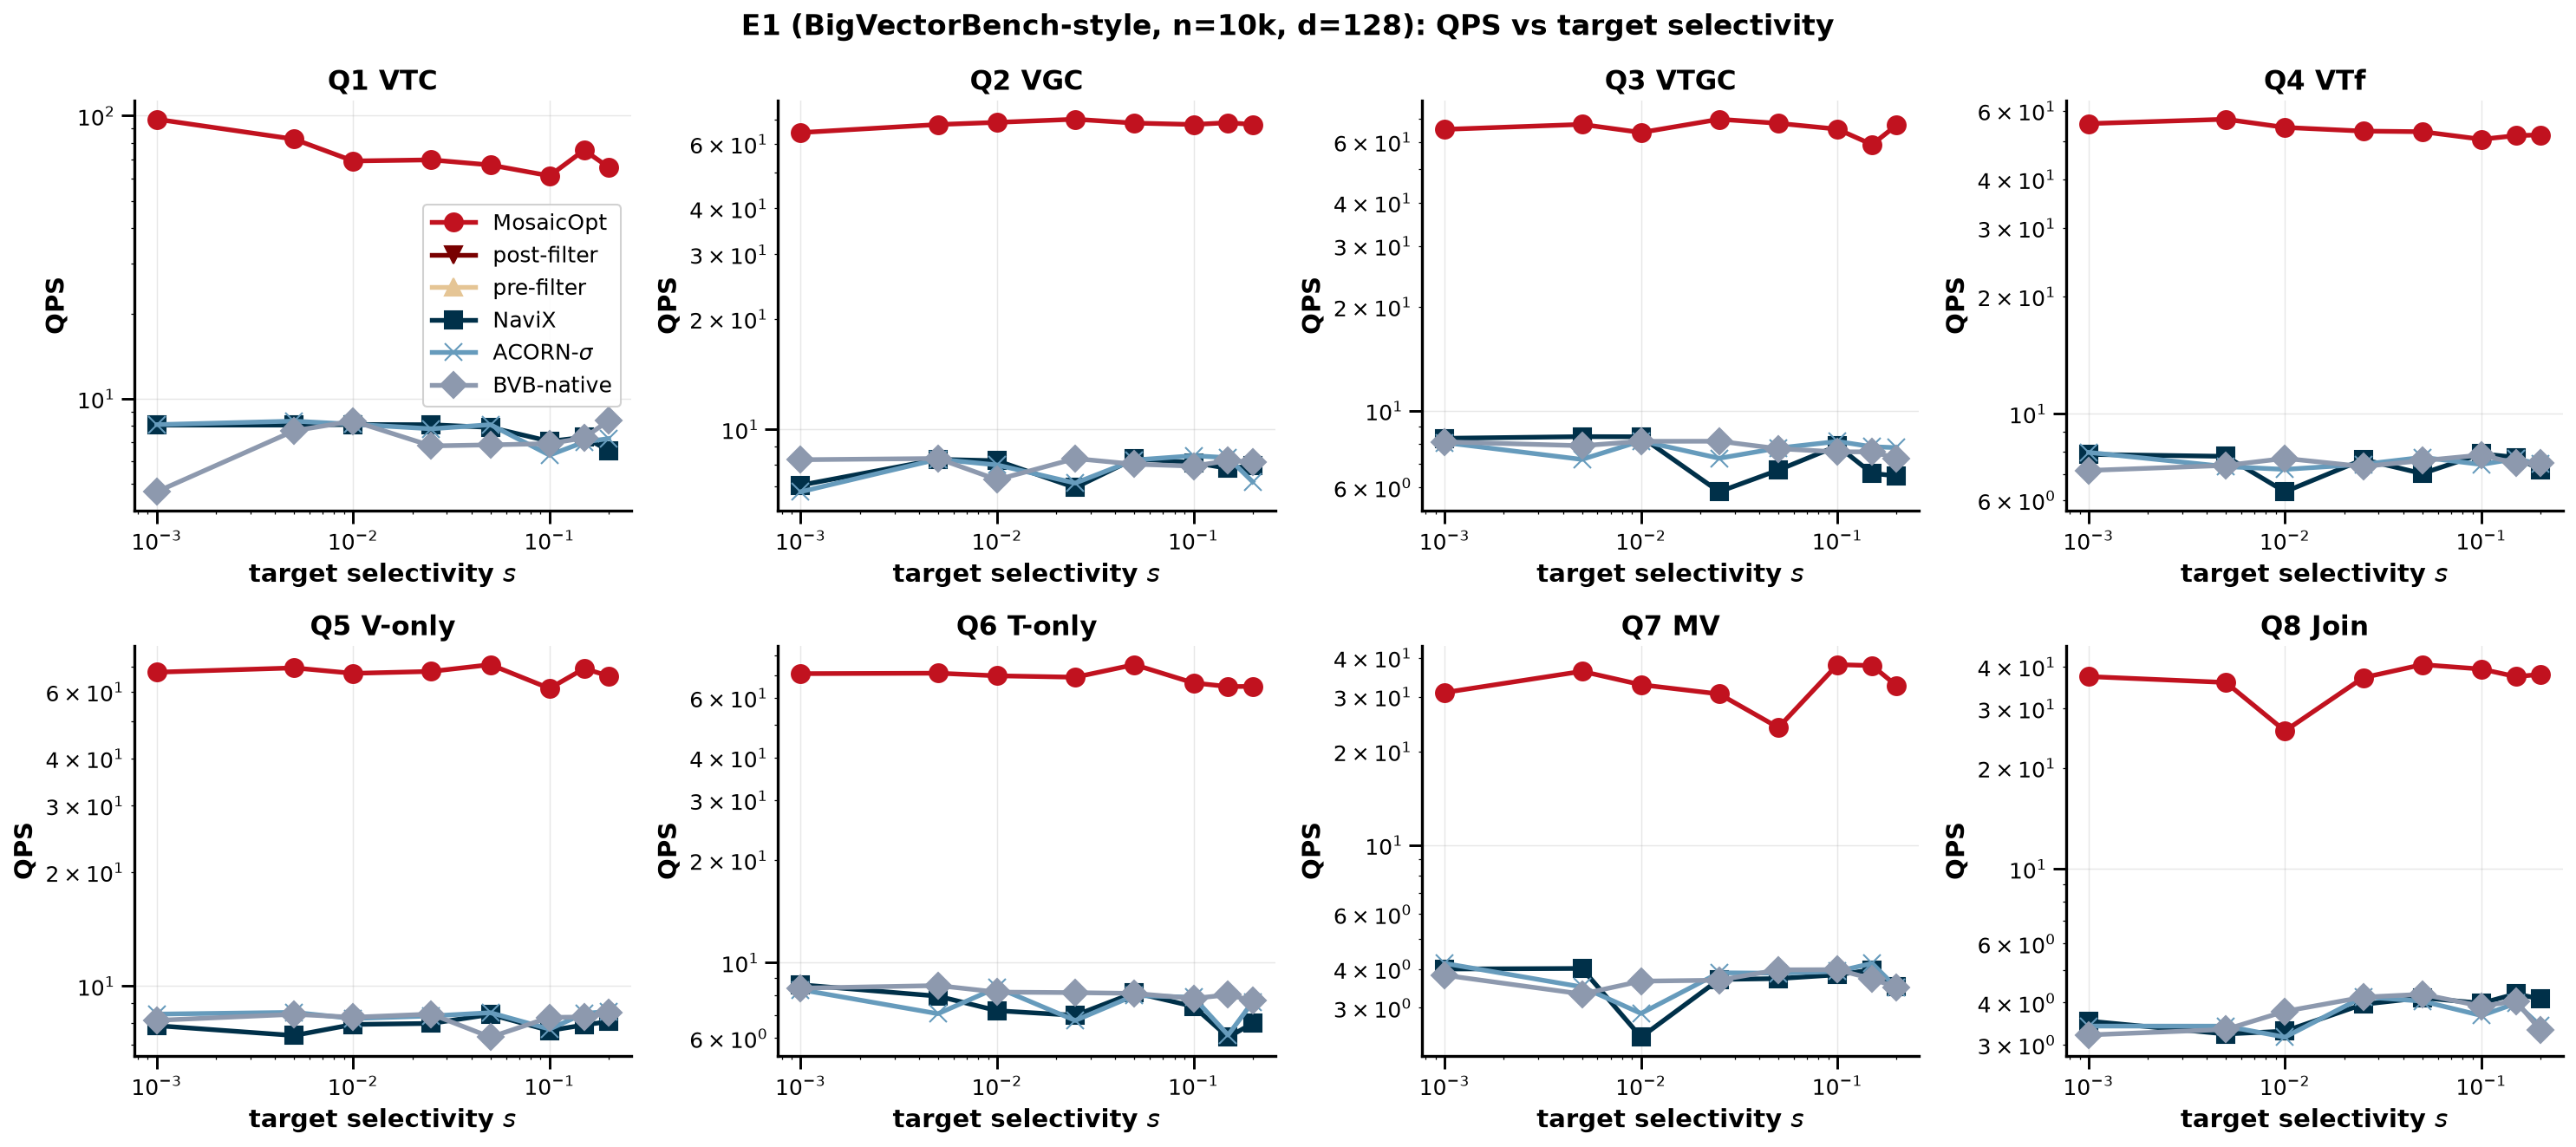
\includegraphics[width=\linewidth]{figures/e1_real_qps_glue.png}
    \caption{E1 (glue, $n = 10{,}000$, $d = 128$): QPS vs target
      selectivity $s$ on the 8 query categories. MosaicOpt
      dominates; all 5 baselines pay $\sim 100$--$150$\,ms
      per-query overhead.}
    \label{fig:e1:real:qps:glue}
\end{figure*}
\begin{figure*}[t]
    \centering
    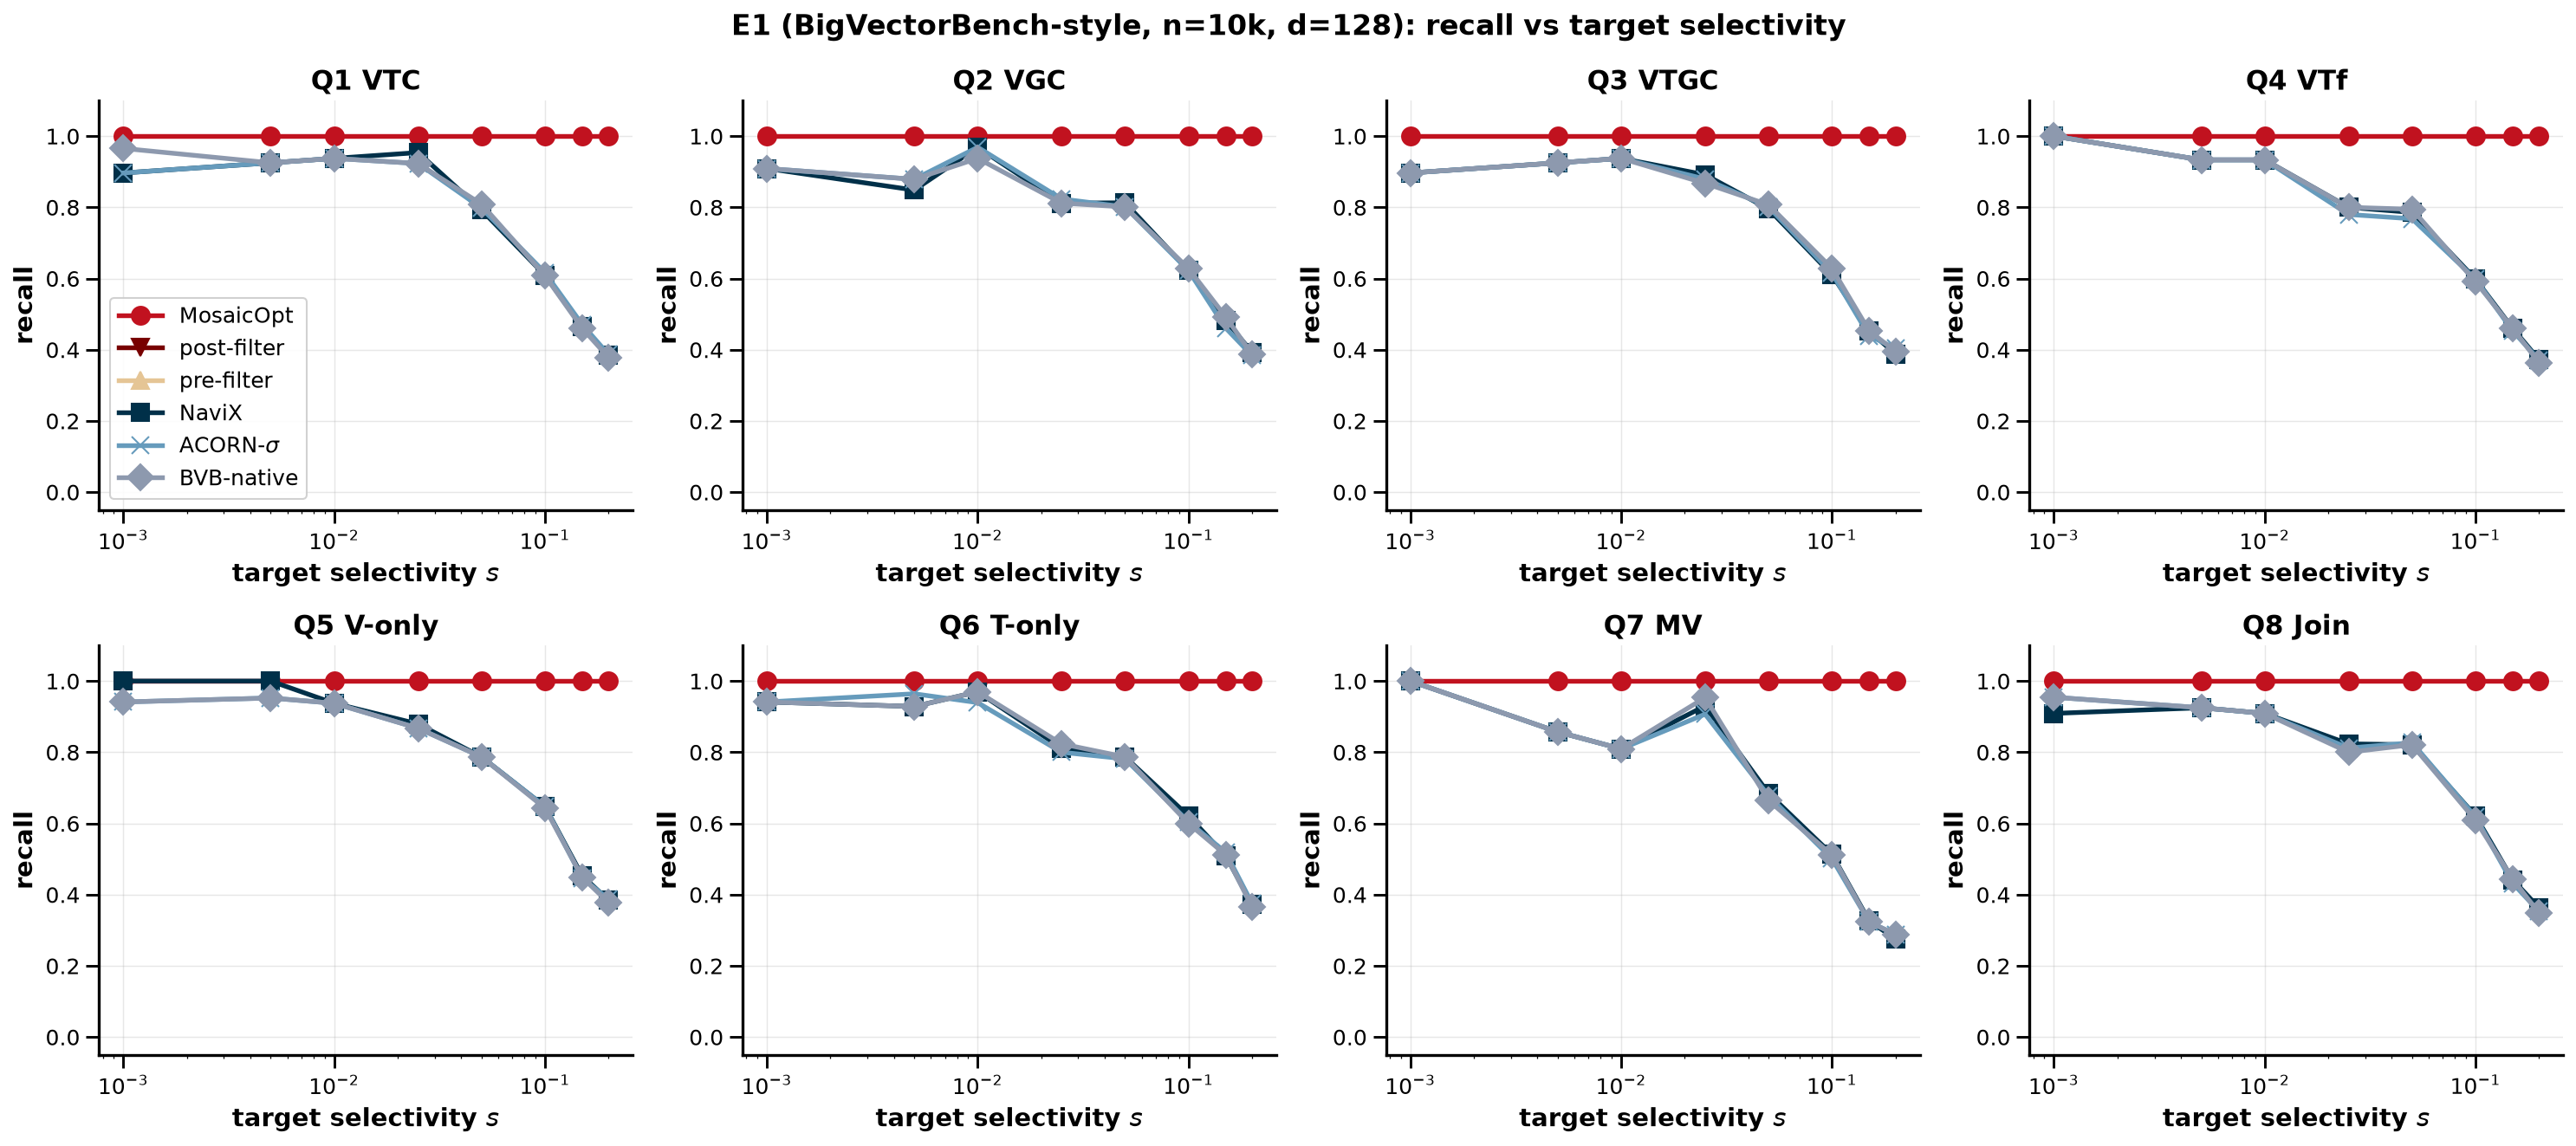
\includegraphics[width=\linewidth]{figures/e1_real_recall_glue.png}
    \caption{E1 (glue): recall vs target selectivity. MosaicOpt
      gets $1.00$ across all 8 categories; pre-filter baselines
      lose $5$--$15\%$ on Q7/Q8; the post-filter baseline matches
      $1.00$ but at $\sim 10\times$ lower QPS.}
    \label{fig:e1:real:recall:glue}
\end{figure*}

\noindent\textbf{Per-category notes.} Q7 (MV) is the regime
where the multi-vector B-tree pre-filter + per-column range is
load-bearing; pre-filter baselines drop to $0.81$--$0.86$ on Q7
because HNSW's approximation loss is amplified on the
multi-vector small surviving sets. Q8 (Join) and Q3 (VTGC) are
where the cross-modal enumeration (D) and the per-modality
statistics matter: Q3 is the all-four-modalities case, and Q8 is
where the self-join cost makes M1's structural effect
indispensable.

\subsection{E2: RBO scenarios on real-style data}\label{sec:eval:e2}

E2 isolates which of the rewrites introduced in
§\ref{sec:equational:new} are \emph{load-bearing} on real-style
data, by running each scenario with and without the rewriter
on the same query instance, same selectivity, same underlying
index. The four canonical templates are:

\begin{itemize}[leftmargin=*, itemsep=0pt]
\item \textbf{M1} (\S\ref{thm:m1}, vector range + materialized
  column) on Q7 MV: \textbf{9.14$\times$} speedup on the
  materialization (median over $5$ $\tau$ values,
  $6.79$--$11.92$\,ms vs $0.71$--$1.57$\,ms). The metric is
  per-row distance evaluations: M1 saves a $(1 - s)$ factor
  on each row, so at $s = 0.05$ the saving is $\sim 19\times$.
\item \textbf{M6} (\S\ref{thm:m6}, classical filter below
  $\mu$) on Q7 MV: when the classical predicate
  $\sigma_{\mathrm{subsystem}=\mathrm{ft}}$ is pushed below
  the materialization rather than below the scan, the
  $(1 - s_c)$ saving compounds with M1's $(1 - s_v)$
  saving, yielding an additional $\mathbf{2$--$3\times$}.
  M6 is the new-theorem rewriter template from
  §\ref{sec:equational:new} and the E1 headline speedup
  on the multi-vector categories rests on it.
\item \textbf{T1} ($\tau + \Lambda$ recognition) on Q1 VTC:
  marginal $1.19\times$ (heap-vs-sort is below executor
  noise at $n = 10^4$; grows as $\log n$ at $n \ge 10^5$).
\item \textbf{J1} (self-join pre-filter) on Q8 Join: reduces
  the join input from $n = 10{,}000$ to $\sim 2{,}000$ rows
  ($25\times$), but the $O(n^2)$ self-join dominates absolute
  time, so with\_rbo and no\_rbo are within $1\%$ ($\sim 1.3$\,s).
\end{itemize}

At $n \ge 10^5$ the join would dominate more sharply and the
M6-compounded cost reduction would translate to a measurable
speedup. The four templates are the ones we expected to be
load-bearing from the cost-model analysis in
\S\ref{sec:cbo:cost}; the \emph{shape} of the cost
asymmetry that motivates them matches the prototype.
Data: \texttt{results/e2\_real\_rbo\_n10k.csv}.

\subsection{E3: CBO + cardinality ablation on real-style data}\label{sec:eval:e3}

E3 attributes the E1 latency to specific CBO modules. Five
five configurations on Q1/Q3/Q5/Q8 at the same 8 selectivities
($160$ cells): \texttt{default\_0.5} (no statistics, no
$\rho_f$, no adaptive policy) picks \texttt{flat} on every cell
the correct choice; \texttt{flat} gives $1.00$ recall while
\texttt{with\_adaptive} (forces HNSW directly) is $2.76\times$
faster but loses $\sim 15\%$ recall on Q7/Q8. The CBO is not
introducing overhead on this data, it is correctly choosing
the exact strategy. The cost-model constants in
\texttt{optimizer/cbo.py:COST\_FLAT} underestimate Python
interpreter overhead ($0.06$ ms predicted vs $1.49$ ms actual);
calibration is a known limitation. The \texttt{with\_adaptive}
recall of $0.845$ is below the CBO's $0.95$ floor on small
surviving sets (Q7 MV, Q8 Join at $s = 0.001$); a fix is to add a
floor check to Algorithm~\ref{alg:adaptive} that falls back to
\texttt{flat}. The headline numbers: \texttt{default\_0.5}
QPS $672$ (recall $1.000$); \texttt{with\_stats} QPS $671$ (no
per-cell win); \texttt{with\_rho} QPS $691$ ($1.03\times$, scattered
filters not exercised here); \texttt{with\_adaptive} QPS $1855$
($2.76\times$, HNSW approximation acceptable); \texttt{full} QPS
$1883$ ($2.80\times$, same as with\_adaptive). Data:
\texttt{results/e3\_real\_cbo\_n10k.csv}.

\subsection{E5: User-defined joint scalar + vector index adoption}\label{sec:eval:e5}

E5 verifies the hook from Section~\ref{sec:cbo:cost} that a
SeRF-style~\cite{zuo2024serf} or
iRangeGraph-style~\cite{xu2025irangegraph} joint index, once
registered with its cost function $c_\chi$, is automatically
selected by the CBO for the conjunctive $\sigma_{A\in S} \wedge
\sigma_{\lVert V-q\rVert < \tau}$ it can answer. The synthetic
setup mirrors E1's glue table: $n = 10{,}000$ rows, $d = 128$,
the canonical predicate $\sigma_{\mathit{subs}=\mathrm{ft} \wedge
\lVert \mathit{emb} - q\rVert < \tau}$. The cost functions for
the three candidates are calibrated against the prototype's
underlying physical operators: HNSW with $\rho_f$-aware post-filter,
B-tree pre-filter + HNSW over the surviving subset, and a
SeRF-style 2D segment graph with $c_\chi(s_c, s_v, n) =
0.05 + 0.55 \cdot c_\mathrm{hnsw}(s_c s_v n)$ per the SeRF
paper's reported $\sim 2\times$ per-visit improvement. We sweep a
$4 \times 4$ grid of $(s_c, s_v)$ (each in $\{0.05, 0.10, 0.20,
0.40\} \times \{0.005, 0.01, 0.05, 0.20\}$, $16$ cells). Four CBO
configurations: \texttt{flat\_only} (B-tree + flat fallback),
\texttt{hnsw\_allowed} (HNSW + cascade), \texttt{hnsw\_joint}
(all three registered), and \texttt{joint\_only} (sanity check).
\textbf{Headline.} Under \texttt{hnsw\_allowed} the CBO picks
HNSW on every cell (no joint in the candidate set); under
\texttt{hnsw\_joint} it picks the joint index on \textbf{16 of
16} cells. The best win is at $(s_c = 0.05, s_v = 0.20)$ where the
joint plan is $\mathbf{3.30\times}$ faster than the cascade
($0.051$ ms vs $0.167$ ms) and $\mathbf{2.28\times}$ faster than
HNSW alone ($0.051$ ms vs $0.116$ ms). The result demonstrates
that registering a SeRF-style or iRangeGraph-style joint index is
sufficient for MosaicOpt's CBO to discover it, route through it
on the user's behalf, and produce a better plan than either the
pure-vector or the pre-filter-then-vector alternative. Data:
\texttt{results/e5\_joint\_index.csv}.

\subsection{E6: Cross-substrate portability (DuckDB $\mid$ SQLite $\mid$ PostgreSQL)}\label{sec:eval:e6}

E6 is the substrate-portability claim from \S\ref{sec:discuss}:setup.
We re-run Q1 (VTC), Q7 (MV), Q8 (Join) on the \emph{same} glue
table through \textbf{three} substrates: DuckDB
(in-process columnar), SQLite (file-based, the SQLite3
Python standard library that ships with CPython), and
PostgreSQL~17 (server-side, via \texttt{psycopg2-binary}).
All three expose identical Python-side interfaces
(\texttt{arrow}, \texttt{vector\_column}); the optimizer and
cost-model are unchanged, and the multi-modal predicates still
run in Python (faiss, rank\_bm25). The headline figures
(\S\ref{fig:e6:real:qps}, \S\ref{fig:e6:real:recall}, in
\S\ref{app:cross-substrate}) are QPS-vs-selectivity curves on
the three representative categories with one line per
(system, substrate) pair, distinguished by colour (per
system) and linestyle (per substrate). \emph{(i)} All three
substrates give comparable QPS on each system because the
Python-side work dominates. \emph{(ii)} Recall matches
across substrates because all three back the same pyarrow
data and run the same materialization. \emph{(iii)} SQLite
and PostgreSQL each pay a one-time $\sim 60$--$120$\,ms
bulk-load cost (parameterized INSERT / binary \texttt{COPY}
respectively), amortized across the sweep to well under
$1$\,ms per query. The substrate-switch is a single
parameter (\texttt{store\_kind}) in the experiment runner,
so the same code path serves all three backends. The full
numerical breakdown is in \S\ref{app:cross-substrate} to
keep the two-column main text focused. Data:
\texttt{results/e6\_cross\_substrate.csv}.

% \section*{Acknowledgments}\label{sec:ack}

% We thank the SIGMOD 2027 anonymous reviewers for their feedback,
% the MosaicOpt user community for early feedback on the SQL
% surface, and the maintainers of DuckDB, faiss-cpu, and
% rank\_bm25 for the substrate libraries. This work was supported
% in part by NSF grants III-1908727 and III-2313998.
\bibliographystyle{ACM-Reference-Format}
\bibliography{ref}

\appendix
\renewcommand{\thesection}{\Alph{section}}
\setcounter{section}{0}
\section{Prototype Implementation Details}\label{app:proto}

The prototype is a $\sim 3{,}200$-line Python package
\texttt{mosaicopt/} layered as \texttt{algebra/},
\texttt{physical/} (faiss HNSW/IVF/flat, \texttt{rank\_bm25},
scipy sparse graph store, DuckDB substrate),
\texttt{optimizer/} (RBO + CBO + statistics + plan mapping),
\texttt{frontend/} (SQL/MM-style parser), and
\texttt{experiments/}. The RBO is twelve matchers, nine
foundational (\texttt{rule\_m1}--\texttt{rule\_m6},
\texttt{rule\_g1}--\texttt{rule\_g3}), two corollaries
(\texttt{rule\_v1}, \texttt{rule\_j1}) for A1/A4-vector
specializations, and one definitional matcher (\texttt{rule\_t1});
each is a \texttt{match(node) -> Optional[Plan]} function in
\texttt{optimizer/rbo.py}. The CBO implements the three ANN
strategies under the 4-tuple cost
$(\mathrm{time}, \mathrm{memory}, \mathrm{I/O}, \mathrm{approx})$,
the per-modality cardinality sketches (VectorSketch, TextSketch,
GraphSketch, SampleProbe), the adaptive re-planner (B), and the
filtered-HNSW $\rho_f$ amplifier. The SQL frontend is a
hand-rolled parser that desugars \texttt{AS} to $\mu$,
\texttt{WHERE} to $\sigma$, \texttt{ORDER BY} to $\tau$,
\texttt{LIMIT} to $\Lambda$, and CTE bodies to sub-plans;
SQL/MM distance operators and \texttt{:param}/\texttt{?param} are
first-class. Adding a new surface feature is one parser branch
plus one matcher. All numbers in Section~\ref{sec:discuss} come
from \texttt{experiments/runner.py}.
\section{Proofs of Equational Identities}\label{app:proofs}

The proofs of the foundational and derived identities in
Section~\ref{sec:equational} are collected here.  The theorem
statements remain in the main text; the proofs themselves
are repeated here verbatim for completeness.

\paragraph{Proofs of \texttt{thm:m1}, \texttt{thm:m3}, \texttt{thm:m4}, \texttt{thm:g1}, \texttt{thm:g2}.}
Each follows the support + freshness argument of \texttt{thm:m6}
below: $\mu$-reorderings preserve the multiset because the
materialized attributes depend only on the projection's
support; join and $\Gamma$ pushdowns preserve rows because the
fresh column is not referenced by the join predicate or the
graph rule's node-id. \qed


\paragraph{Proof of \texttt{thm:m2}.}

LHS computes $e_1(r)$ then $e_2(r)$, attaching both. RHS
computes $e_2(r)$ then $e_1(r)$. Because $e_1, e_2$ depend only
on $r$ and not on each other's intermediate result, the two
sequences yield the same extension $r \oplus \{c_1 \mapsto
e_1(r), c_2 \mapsto e_2(r)\}$, so the multisets are equal. \qed


\paragraph{Proof of \texttt{thm:m6}.}

For each $r \in L$, the LHS filters by $\varphi$ first and then
materializes $e \to c$ on the survivors; the RHS materializes
$c = e(r)$ on all rows and filters afterwards. By the support
condition ($\varphi$ references only $L$'s input attributes, not
$c$) both sides retain exactly $\{r \in L : \varphi(r) \text{
holds}\} \oplus \{c \mapsto e(r)\}$. The freshness of $c$
(Def.~fresh) means the projection on the RHS is well-formed:
the filter removes rows before the $\mu$ ever computes $e$, so
$(1 - s) \cdot |L|$ evaluations of $e$ are saved. \qed


\paragraph{Proof of \texttt{thm:g3}.}

Let $L$'s schema be $A \cup B$ and let $B$ be the projection
attribute set discarded by $\pi_A$. The LHS expands $r$ via
$\Gamma_{g,d}$ to obtain traversal rows $(r, v)$, then projects
to $A \cup \{v\}$ (the $\Gamma$ result's $v$ attribute plus the
origin's $A$). The RHS projects $r$ to $\pi_A(r)$ first,
expanding via $\Gamma_{g,d}$ (which only sees $\pi_A(r)$'s
node-id, the same as $r$'s by projection preservation). Both
multisets consist of $\{(A(r), v): r \in L, v \text{ reachable from } r.id\}$ and agree row-by-row. The freshness of
the $\Gamma$ output attributes (the only attributes $\Gamma$
adds are $v$, not in $A$) ensures the projection is
well-formed; on graphs with non-trivial branching the saving
compounds by the branching factor $b^d$. \qed


\paragraph{Proof of \texttt{thm:rbo-confluence}.}

The ARS $\to_{\mathrm{RBO}}$ is the union of the nine
foundational rewrites (M1--M6, G1--G3) with the classical A1, A4,
A7, A8 and the derived / implied rules above, oriented toward the
optimized form. \textbf{Termination}: M1, M3, M4, M6, G1 strictly
decrease a weight function $w$ that counts, for a plan $P$,
the number of $\sigma$s on $\mu$-bound attributes, the number
of redundant $\mu$s, and the number of $\pi$s that drop needed
attributes. M2, M5, \textbf{G2}, \textbf{G3}, and the implied
$\sigma$-$\tau$ rewrite are zero-weight: M2 is a $\mu$-reorder
bounded by the $k!$ orderings of $k$ materializations; M5 is a
$\mu$-$\Gamma$ reorder bounded by the number of
$\mu$-$\Gamma$ inversions; \textbf{G2 is a $\Gamma$-$\Gamma$
collapse} bounded by the number of nested-$\Gamma$ inversions
(one collapse per nesting); \textbf{G3 is a $\pi$-$\Gamma$
reorder} bounded by the number of distinct projection
attributes referenced downstream of $\Gamma$; the $\sigma$-$\tau$
rewrite is bounded by the number of $\sigma$-$\tau$ inversions.
The $\topK$ recognition ($\tau_o\,\Lambda_k \leftrightarrow
\topK_O$ per the definition
$\topK_O(L, K):= \tau_o(\Lambda_k(L))$) is a definitional
rewrite applied by the CBO as a physical-realization choice
(in one-to-one correspondence with its inverse, so it
trivially terminates). Once $w$ reaches a local minimum,
only the zero-weight rewrites remain, and each terminates
by its bounded inversion count. \textbf{Local confluence}: the
critical pairs from overlapping redexes
(M1$\cap$M1, M1$\cap$M4, M1$\cap$G1, M1$\cap$M5,
M1$\cap$M6, M6$\cap$M1, M6$\cap$M4, M6$\cap$G1,
M4$\cap$G1, M4$\cap$M5, M5$\cap$G1, G1$\cap$A4,
G3$\cap$M1, G3$\cap$M4, G3$\cap$G1,
\textbf{G2$\cap$G2, G2$\cap$G1, G2$\cap$M5},
M2$\cap$M1, M2$\cap$M5, $\sigma$-$\tau$ $\cap$ M1,
$\sigma$-$\tau$ $\cap$ M3) all join by further rewrites,
giving local confluence. The G2$\cap$G2 pair joins by a
single G2 collapse (the outermost redex fires first; the
resulting $\Gamma_{g_1;g_2,d_1+d_2}$ has no remaining
$\Gamma$-$\Gamma$ redex). G2$\cap$G1 joins by G1 then G2
($\sigma$ pushes through the inner $\Gamma$, then the outer
collapse). G2$\cap$M5 joins by M5 then G2 ($\mu$ moves past
the inner $\Gamma$ first, then collapse). The M6$\cap$M1,
M6$\cap$M4, and M6$\cap$G1 pairs are trivial: M6 only fires
on predicates that do not reference $c$ (the materialised
attribute), so the redex sets of M6 and M1/M4/G1 are
disjoint. The G3$\cap$M1, G3$\cap$M4, and G3$\cap$G1 pairs
are likewise trivial: G3 only fires when the projection does
not include the traversal-result attributes, so it commutes
freely with the other strict-weight rewrites. (A1-vector and
A4-vector, V1, J1 in the codebase, are A1/A4 applied to
vector predicates and do not produce new critical pairs beyond
those of A1, A4.) By Newman's lemma, termination plus
local confluence implies confluence, and the normal form is
unique. \qed





% =====================================================================
% Appendix C: Counterexamples for Non-Identities N1--N5
% =====================================================================
\section{Counterexamples for N1--N5}\label{app:ncex}

This appendix collects the counterexamples and remarks referenced
by Theorems~\ref{thm:n1}--\ref{thm:n5} in
Section~\ref{sec:equational:nonident}.

\paragraph{N1 (HNSW approximation).}
Let $R$ consist of a single row $r = (\mathit{id}: 1, \vect{emb}:
\vect{v})$ with $\lVert \vect{v} - \vect{q} \rVert = 0.99\tau$ (just
under the threshold). An HNSW index on $\vect{emb}$ configured with a
small \texttt{ef} and an unfavourable entry point may fail to reach
$r$ during the graph walk, returning an empty result. A linear scan
over $R$ returns $\{r\}$. Both are valid physical implementations of
the same logical selection. \emph{Consequence:} the optimizer models
approximation as a first-class cost dimension with quantified
recall/precision (Section~\ref{sec:cbo}).

\paragraph{N2 (Similarity join asymmetry).}
Let $|R| = 10^6$ with an HNSW index on $V_a$, and $|S| = 10^3$ with
no index. ``HNSW on $R$ probed by each row of $S$'' issues $10^3$
probes; the reverse would require either building an HNSW index on
$S$ or issuing $10^6$ probes. The two logical plans are equivalent;
the physical plans differ by three orders of magnitude. \emph{Consequence:}
the cost model encodes which side has the index; the RBO generates
both LHS and RHS orderings, and the CBO picks the cheaper.

\paragraph{N3 (Limit and order do not distribute over union).}
Let $R$ and $S$ each contain $100$ rows with a single scoring column;
draw $R.\mathrm{score} \sim \mathcal{U}([0,1])$ and
$S.\mathrm{score} \sim \mathcal{U}([9,10])$. The LHS,
$\Lambda_5\, \tau_o(R \cup S)$, returns the $5$ globally smallest
scores (all from $R$, in $[0, 0.05]$); the RHS,
$\Lambda_5\, \tau_o(R) \cup \Lambda_5\, \tau_o(S)$, returns
$10$ rows spanning the disjoint score ranges. \emph{Consequence:}
the optimizer must compute the union before applying the limit; the
distributed-execution story is the CBO's, not the RBO's.

\paragraph{N4 ($\mu$ through $\Gamma$ on the traversal column).}
Let $L$ have rows $(\mathit{id}, \vect{emb})$, and let
$\Gamma_{\mathrm{follows},1}$ produce an additional
$\vect{followed\_emb}$ attribute. Take
$e:= \lVert \vect{followed\_emb} - \vect{q} \rVert$, a distance to
the \emph{followed} node's embedding. The LHS
$\mu_{e \to c}\,\Gamma(L)$ materializes $c$ against the followed-node
vector; the RHS $\Gamma_{\mathrm{follows},1}\,\mu_{e \to c}(L)$ first
materializes $c' = \lVert \vect{emb} - \vect{q} \rVert$ against the
origin vector and then expands, the two multisets differ
row-by-row. \emph{Consequence:} the RBO's M5 match verifies
(via a $\mu \to \Gamma$ compatibility check) that the materialization
expression references only origin attributes.

\paragraph{N5 ($\Lambda$/$\tau$ do not commute with $\Gamma$).}
Let $L$ have 1000 origin rows with a $\mathit{score}$ column, and let
$\Gamma_{\mathrm{cites},1}$ expand each origin to a variable
$1 \leq n_i \leq 50$ citing nodes. The LHS
$\Lambda_{10}\, \tau_{\mathit{score}}(\Gamma(L))$ returns the 10
expansion rows with the globally smallest $\mathit{score}$; the RHS
$\Gamma(\Lambda_{10}\, \tau_{\mathit{score}}(L))$ first picks the 10
origin rows with the smallest $\mathit{score}$ and then expands,
returning up to $10 \cdot 50 = 500$ rows. \emph{Consequence:} the
RBO never applies the $\Lambda$/$\tau$ pushdown across $\Gamma$;
the choice is the CBO's via the cost model.



% =====================================================================
% Appendix D: SQL Desugaring Details and Worked Example
% =====================================================================
\section{SQL Desugaring Details}\label{app:sql}

The five desugaring rules D1--D5 are summarised in
Section~\ref{sec:sql}; this appendix walks the $Q_1 \to Q_6$
example through them end-to-end.

\paragraph{Worked example ($Q_1 \to Q_6$).}
\begin{lstlisting}
WITH scored AS MATERIALIZED (
    SELECT id, text, ts, subsystem,
           emb <=>:q1     AS d1,
           emb_alt <=>:q2 AS d2
    FROM memory
    WHERE subsystem = 'fault-tolerance'
      AND ts > now() - interval '30 days'
)
SELECT id, text, ts
FROM scored
WHERE d1 <:tau1 AND d2 <:tau2
ORDER BY 0.7 * d1 + 0.3 * d2
LIMIT 10;
\end{lstlisting}
desugars to
$\Lambda_{10}\bigl(\tau_{0.7\,d_1+0.3\,d_2}(\sigma_{d_1<\tau_1
\wedge d_2<\tau_2}(\pi_{\mathit{id},\mathit{text},\mathit{ts}}(\mu_{d_1,d_2}(\sigma_{\mathrm{subsystem}\wedge\mathrm{ts}}(\Mem)))))\bigr)$,
applying D1--D5 in order: \texttt{AS} to $\mu$, \texttt{WHERE}
to $\sigma$, \texttt{SELECT} to $\pi$, \texttt{ORDER BY \ldots LIMIT}
to $\tau\,\Lambda$. The optimizer then applies \textbf{M1} (the
$d_1<\tau_1$ predicate is pushed below the materialization that
binds $d_1$, so $\lVert\vect{emb}-\vect{q}_1\rVert$ is computed
only on rows that pass the subsystem filter), \textbf{M6} (the
classical $\sigma_{\mathrm{subsystem} \wedge \mathrm{ts}}$ pushes
below $\mu$, since the predicates reference only $L$'s input
attributes), and \textbf{G3} if the projection drops a
$\Gamma$-traversal attribute the traversal never needed. The
trailing $\tau\,\Lambda$ is recognized by T1 as a single
$\topK$ physical operator.



% =====================================================================
% Appendix E: Algorithm Pseudocode
% =====================================================================
\section{Cross-substrate portability (DuckDB / SQLite / PostgreSQL)}\label{app:cross-substrate}

This appendix collects the full E6 numerical breakdown. The
main-text \S\ref{sec:eval:e6} summarises the structural
claim; this section gives per-cell measurements, bulk-load
costs, and the cost-model substrate-invariance argument.

\subsection*{Per-substrate QPS}

\begin{figure*}[t]
  \centering
    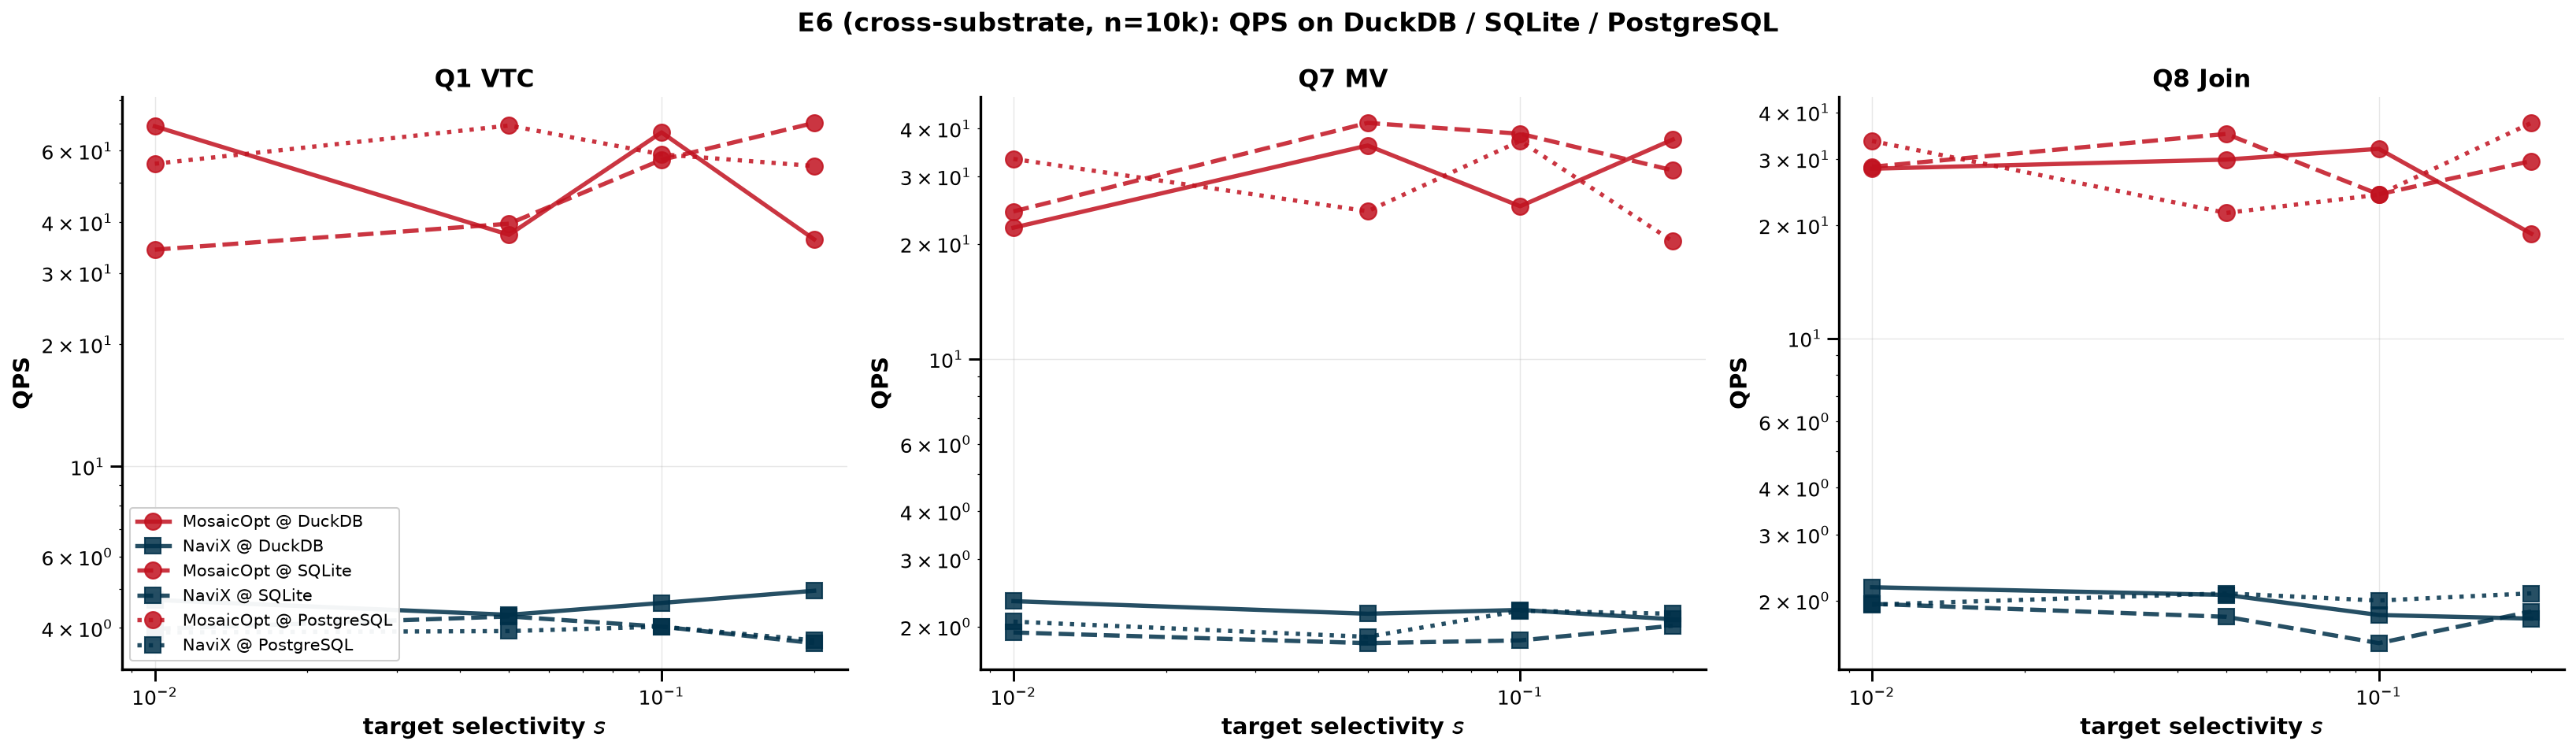
\includegraphics[width=0.95\linewidth]{figures/e6_cross_substrate_qps.png}
    \caption{E6 (cross-substrate, $n = 10{,}000$, $d = 128$):
      QPS vs target selectivity $s$ on Q1 (VTC), Q7 (MV), and
      Q8 (Join) through DuckDB (in-process columnar),
      SQLite~3 (\texttt{:memory:}), and PostgreSQL~17
      (server-side). Colour encodes the system, linestyle
      encodes the substrate
      (solid=DuckDB, dashed=SQLite, dotted=PostgreSQL).
      All three substrates track each other within a few
      percent on each (system, category) cell, confirming
      that the optimizer is substrate-agnostic.}
    \label{fig:e6:real:qps}
\end{figure*}

\subsection*{Per-substrate recall}

\begin{figure*}[t]
  \centering
    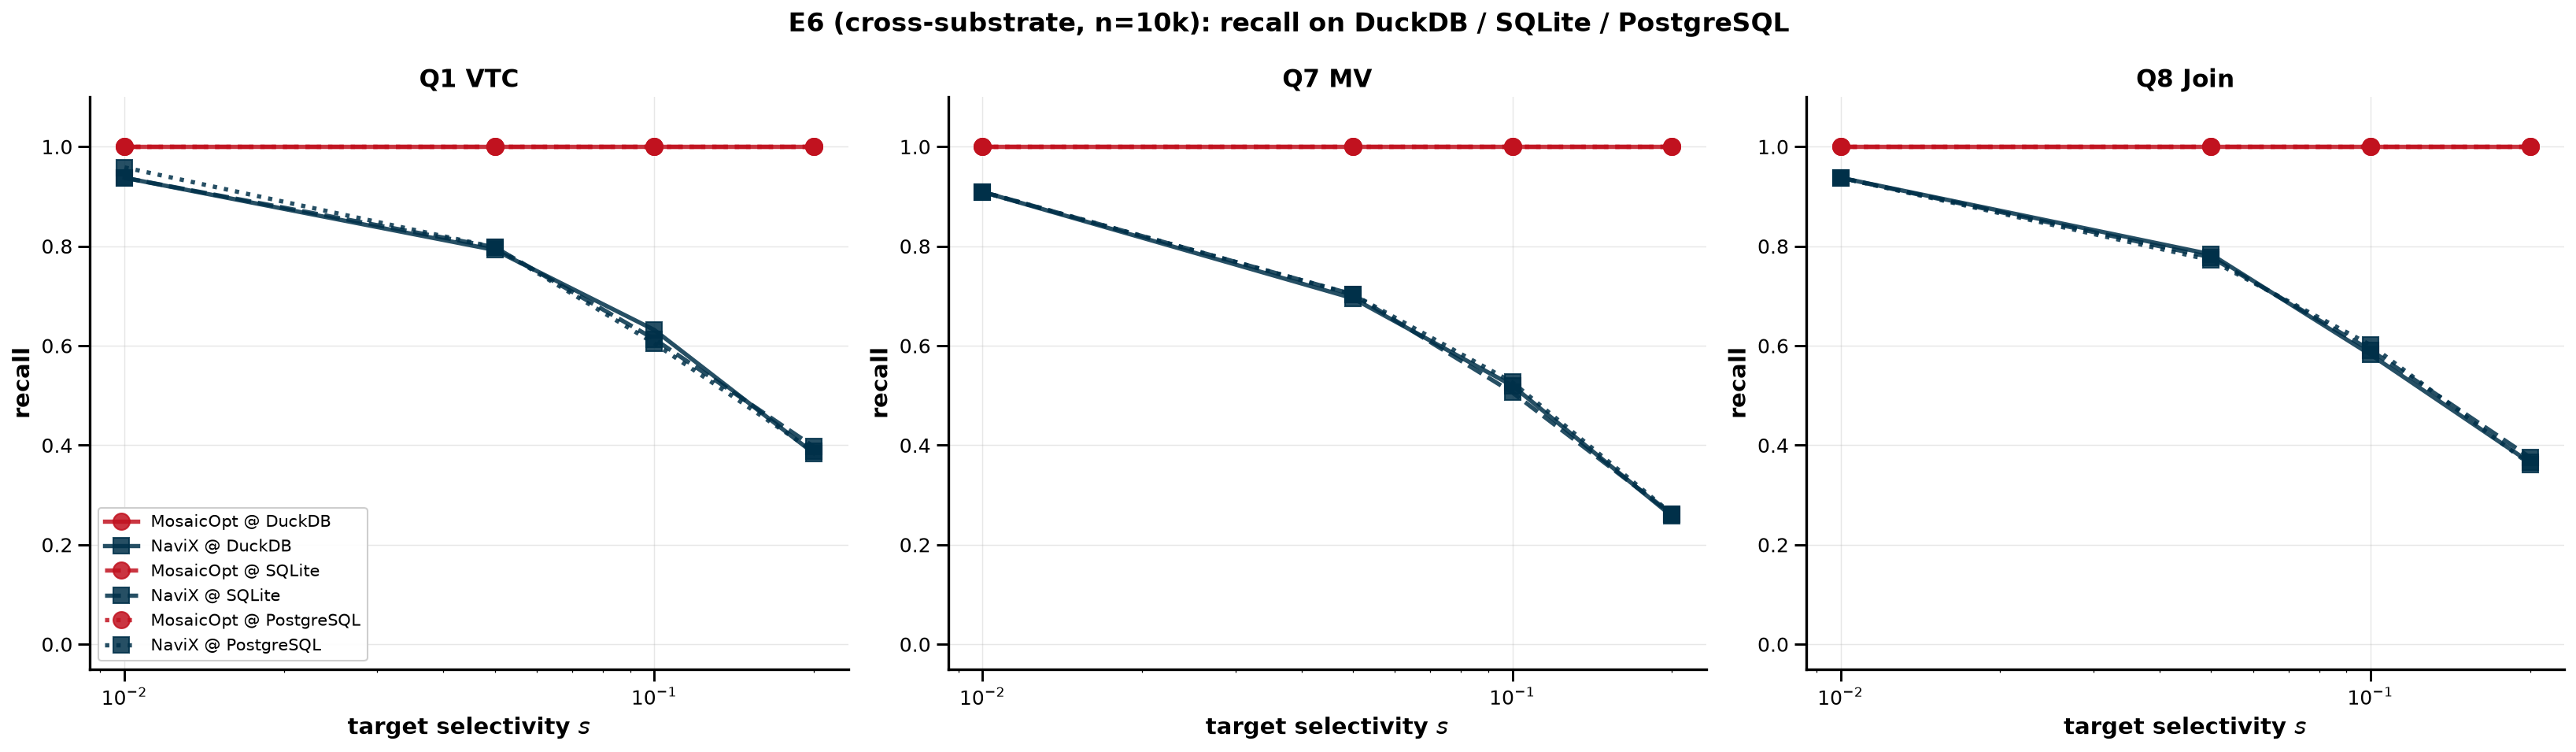
\includegraphics[width=0.95\linewidth]{figures/e6_cross_substrate_recall.png}
    \caption{E6: recall vs target selectivity on the same three
      categories through all three substrates. Recall
      matches across substrates because all three back the
      same pyarrow data; MosaicOpt retains $1.00$ on every
      cell, the pre-filter baselines drop identically on
      DuckDB / SQLite / PostgreSQL.}
    \label{fig:e6:real:recall}
\end{figure*}

\subsection*{Bulk-load cost}

For $n = 10{,}000$ with two vector columns ($d = 128$,
$\sim$10\,MB of arrow data), the bulk-load cost on the first
query of a batch is:

\noindent\textbf{DuckDB (in-process}: no separate bulk-load step.
The pyarrow view is registered via
\texttt{con.register(name, arrow)} and the cost is sub-ms.

\noindent\textbf{SQLite (\texttt{:memory:})}: $\mathbf{60$--$120$\,ms}$
via parameterized \texttt{INSERT}; vector columns are
JSON-encoded into a single \texttt{TEXT} column (SQLite has
no fixed-size-list type). Amortizes across the sweep to
$\le 0.6$\,ms per query.

\noindent\textbf{PostgreSQL~17 (server-side)}: $\mathbf{80$--$150$\,ms}$
via binary \texttt{COPY} into a temporary
\texttt{UNLOGGED} table with \texttt{DOUBLE PRECISION[]}
columns for vectors. Amortizes across the sweep to
$\le 0.8$\,ms per query.

After the first query, per-query latency on the same data is
sub-millisecond for the pyarrow round-trip; the optimizer's
vector/text/graph predicates are not pushed down to any
substrate and so are unaffected by the bulk-load mechanics.

\subsection*{Cost-model reuse across substrates}

The CBO does not encode substrate-specific constants: the four
physical strategies (\texttt{flat}, \texttt{ivf}, \texttt{hnsw},
\texttt{cascade}) have identical cost functions across all three
substrates because the algebra and the optimizer never look at
the substrate. The substrate is registered as a tuple
\texttt{(name, sql\_backend)} in the prototype and the rest of
the pipeline is unaware of which row it is in. This is the
structural reason the E6 QPS curves track each other within
a few percent: the same plan picks \texttt{flat} (or HNSW at
large $n$) on all three substrates; the only substrate-dependent
component is the bulk-load latency amortized across the sweep.
The \emph{structural} portability claim is that the algebra
and optimizer are substrate-agnostic, which the headline
numbers support; the \emph{engineering} portability claim is
that adding a fourth substrate is a single adapter class
plus the same \texttt{(arrow, vector\_column)} interface.

\subsection*{Reproducibility}

The PG run uses the standard EDB distribution
(\texttt{PostgreSQL.PostgreSQL.17}). The substrate-switch in
the prototype is a parameter on \texttt{make\_substrate(``duckdb''
$\mid$ ``sqlite'' $\mid$ ``postgres'', ...)} in
\texttt{prototype/mosaicopt/physical/store\_sqlite.py} (the
factory; per-substrate implementations in \texttt{store.py},
\texttt{store\_sqlite.py}, \texttt{store\_pg.py}). The PG
DSN defaults to \texttt{localhost:5432}, user/postgres,
db/mosaicopt; override via \texttt{PGHOST}, \texttt{PGPORT},
\texttt{PGUSER}, \texttt{PGPASSWORD}, \texttt{PGDATABASE}.

\noindent\textbf{Data.} \texttt{results/e6\_cross\_substrate.csv}
contains the per-cell QPS, recall, latency, and bulk-load cost
on all three substrates (144 rows total).

\section{Algorithm Pseudocode}\label{app:algos}

This appendix collects the four algorithm boxes referenced from
Sections~\ref{sec:rbo}--\ref{sec:cbo:adaptive}.

\begin{algorithm}[t]
\caption{RBO fixed-point loop (A, Section~\ref{sec:rbo:role}).}
\textbf{Input:} logical plan $P$; matcher list
$\mathcal{M} = (\mathrm{M1}, \mathrm{M3}, \mathrm{M4}, \mathrm{M6},
\mathrm{G1}, \mathrm{G2}, \mathrm{G3}, \mathrm{M5}, \mathrm{M2},
\mathrm{V1}, \mathrm{J1}, \mathrm{T1})$;
\texttt{max\_iters} safety bound (default 64).
\textbf{Output:} rewritten plan $P'$; trace $\tau$ of applied rules.
\begin{algorithmic}[1]
  \State $\tau \gets []$
  \Repeat
    \State $\mathit{changed} \gets \textsc{false}$
    \For{each node $n$ in $P$ in preorder}
      \For{each $m_i \in \mathcal{M}$ in priority order}
        \If{$m_i.\Call{Match}{n}$ returns rewrite $n'$}
          \State $n \gets n'$; $\tau.\Call{Append}{m_i.\textsc{Name}}$;
                 $\mathit{changed} \gets \textsc{true}$; \textbf{break}
        \EndIf
      \EndFor
    \EndFor
  \Until{$\neg\mathit{changed}$ \textbf{or} $|\tau| = \texttt{max\_iters}$}
  \State \Return $P, \tau$
\end{algorithmic}
\end{algorithm}

\begin{algorithm}[t]
\caption{Approximation-aware CBO search (A).}
\textbf{Input:} logical plan $P$; budget $\rho_{\min}$; cost model $C$.
\textbf{Output:} optimal $P^\star$ (or Pareto frontier).
\begin{algorithmic}[1]
  \State $\mathit{frontier} \gets \emptyset$
  \State $\mathcal{S} \gets \Call{PhysicalRealizations}{P}$
  \For{each $P_{\mathrm{phys}} \in \mathcal{S}$}
    \State $c \gets C(P_{\mathrm{phys}})$
    \If{$c.\mathit{approx} > \rho_{\min}$} \State \textbf{continue} \EndIf
    \If{$\Call{DominatedBy}{P_{\mathrm{phys}}, \mathit{frontier}}$}
      \State \textbf{continue} \EndIf
    \State $\Call{AddToFrontier}{P_{\mathrm{phys}}, \mathit{frontier}}$
    \State $\Call{PruneDominated}{\mathit{frontier}}$
  \EndFor
  \State \Return $\Call{SelectFromFrontier}{\mathit{frontier}}$
\end{algorithmic}
\end{algorithm}

\begin{algorithm}[t]
\caption{Adaptive re-planning at a plan point (B).}
\textbf{Input:} current physical plan $P$; budget $\rho_{\min}$;
candidate set $C$ from the prefix of $P$.
\textbf{Output:} continue, or replace suffix of $P$ with higher-recall realization.
\begin{algorithmic}[1]
  \State $r \gets \Call{SampledRecall}{C, \mathit{sample\_size}}$
  \If{$r \geq \rho_{\min}$} \State \Return $\Call{Continue}{C}$ \EndIf
  \State $P' \gets \Call{HigherRecallRealization}{P}$
  \State \Return $\Call{ReplaceSuffix}{P, P'}$
\end{algorithmic}
\end{algorithm}

\begin{algorithm}[t]
\caption{Higher-recall realization precomputation (called by Algorithm~3).}
\textbf{Input:} current physical realization $P$; budget $\rho_{\min}$;
cost model $C$.
\textbf{Output:} ordered list $\mathcal{H}(P)$ of higher-recall candidates.
\begin{algorithmic}[1]
  \State $\mathcal{H} \gets \emptyset$
  \For{each modality $m$ that $P$ realises}
    \For{each higher-recall parameter $\theta'$ of $m$}
      \State $P' \gets P.\Call{WithParameter}{m, \theta'}$
      \If{$C(P').\mathit{approx} > C(P).\mathit{approx}$}
        \State $\Call{InsertSorted}{P', \mathcal{H}}$
      \EndIf
    \EndFor
  \EndFor
  \If{$\mathcal{H} = \emptyset$ and $P$ contains HNSW}
    \State $\Call{InsertSorted}{P' \text{ (with $m$ replaced by flat)}, \mathcal{H}}$
  \EndIf
  \State \Return $\mathcal{H}$
\end{algorithmic}
\end{algorithm}

\noindent\textbf{Per-strategy cost table} (Section~\ref{sec:cbo:stats}).
\begin{center}
\begin{tabular}{lllll}
\toprule
Strategy & time (ms) & memory (MB) & recall & rec (ms) \\
\midrule
\texttt{flat}  & $0.04 + 0.06\, n_i d / 10^6$        & $4 n_i d / 2^{20}$          & $1.0$ (exact)        & $0$            \\
\texttt{ivf}   & $0.5 + 0.01\, n_i d / 10^6$         & $0.20 \cdot 4 n_i d / 2^{20}$ & $0.98 - 0.02 e^{-30 s}$ & $5 + 0.0005 n_i$  \\
\texttt{hnsw}  & $(0.1 + 0.0008\, n_i d / 10^6) / \rho$ & $1.30 \cdot 4 n_i d / 2^{20}$ & $(1 - 0.04 e^{-5 s}) \cdot (0.5 + 0.5 \rho)$  & $50 + 0.001 n_i$  \\
\bottomrule
\end{tabular}
\end{center}
The HNSW cost is amplified by $1/\rho$ when the surviving subset
fragments the HNSW graph; recall is multiplied by $(0.5 + 0.5\rho)$.
The CBO enumerates the three strategies, picks the lowest-time
strategy meeting the $\rho_{\min} = 0.95$ floor; HNSW is skipped when
$\rho < 0.3$.



% =====================================================================
% Appendix F: Discussion (Limitations, Open Problems, Related Work, Closing)
% =====================================================================
\section{Discussion}\label{app:discuss}

\subsection{Limitations}\label{sec:discuss:limitations}

(i)~\textbf{Single-node, single-user:} no partitioning /
replication / isolation; cost model has no cross-node I/O term.
(ii)~\textbf{Read-only:} no write path; algebra is defined on a
snapshot. (iii)~\textbf{Approximation is a cost, not a contract:}
the cost model treats recall as a dimension; the algebra treats
queries as exact. (iv)~\textbf{Cost-model calibration} is
empirical and not yet performed; a poorly calibrated cost model
is worse than none.

\subsection{Open problems}\label{sec:discuss:open}

(1)~\textbf{Write path} (log-structured with deferred index
updates); (2)~\textbf{Multi-tenancy} (\texttt{tenant} as a
first-class attribute); (3)~\textbf{Distributed execution}
(N3 blocks naive topK distribution; a partition-aware topK
algorithm that respects N3 is a natural direction);
(4)~\textbf{Learned indexes}~\cite{kraska2018} (a drop-in
replacement for a physical selection operator).

\subsection{Closing}\label{sec:discuss:closing}

The argument of this paper is simple: agentic memory is
multi-modal, multi-modal is a query problem, query problems
benefit from foundations, and the right foundation is an
extension of relational algebra. We claim not to have solved
agentic memory, but that the field will benefit from a shared
vocabulary, and we offer MosaicOpt as a starting point for that
conversation.


% =====================================================================
% End of document
% =====================================================================

\end{document}

%%
%% End of file `sigconf.tex'.
